\chapter{Phase transitions}
\newcommand{\Nphases}{n_{p}}
\section{Phases}
We can generalise  the formalism introduced in statistical physics to incorporate different coexisting phases.

\subsection{Isolated systems}

We begin with isolated systems, where the total volume, total  energy, and the particle number per component is conserved. Let's assume that there are $\Nphases $ coexisting phases, which we enumerate by
($\nu=1,\ldots,\Nphases $) and $\alpha$ components, enumerated by ($j=1,\ldots,\alpha$).
The conditions for isolated systems are therefore
\begin{subequations}\label{eq:constraints}
\begin{align}
\sum_{\nu=1}^{\Nphases } V_{\nu} &= V\\
\sum_{\nu=1}^{\Nphases } U_{\nu} &= U\\
\sum_{\nu=1}^{\Nphases } N_{j\nu} &= N_{j}\;,\text{for } j=1,\ldots, \alpha\;.
\label{eq:constraints:c}
\end{align}
\end{subequations}
Here $V_{\nu}$ ($U_{\nu}$) is the total volume (energy) of the  particles in phase $\nu$.
$N_{j}$ is the total number of particles of component $j$ and $N_{j\nu}$ the number of component
$j$ that is in phase $\nu$. We also introduce the following vectors
%
\begin{align}\label{def:N}
\vv N &= (N_{j=1},N_{j=2},\ldots,N_{\alpha})^{T}\\
\vv N_{\nu} &= (N_{j=1,\nu},N_{j=2,\nu},\ldots,N_{\alpha,\nu})^{T}\;.
\end{align}
%
The entropy as extensive quantity is 
%
\begin{align}\label{eq:}
S(U,V,\vv N) &= \sum_{\nu=1}^{\Nphases } S_{\nu}(U_{\nu},V_{\nu},\vv N_{\nu})\;.
\end{align}
%
For an isolated system (micro-canonical ensemble) the entropy represents the thermodynamic
potential and in equilibrium it has to be maximal. So we have to maximize the entropy based on
the constraints in \eq{eq:constraints}. This is best achieved by Lagrange multipliers, i.e. we define
%
\begin{align}\label{eq:}
{\cal L} &= \sum_{\nu} S_{\nu}(U_{\nu},V_{\nu},\vv N_{\nu})
-\lambda^{V} \sum_{\nu} V_{\nu}
-\lambda^{U} \sum_{\nu} U_{\nu}
-\sum_{j}\lambda^{N}_{j}\sum_{\nu} N_{j\nu}
\end{align}
%
and form the differential
\begin{subequations}\label{eq:}
\begin{align}
d{\cal L} &= \sum_{\nu=1}^{\Nphases } 
\bigg[\frac{\partial }{\partial U_{\nu}}S_{\nu}(U_{\nu},V_{\nu},\vv N_{\nu})\at_{V_{\nu},\vv N_{\nu}} -\lambda^{U}\bigg]dU_{\nu}\\
&\quad +\sum_{\nu=1}^{\Nphases } \bigg[\frac{\partial }{\partial V_{\nu}}S_{\nu}(U_{\nu},V_{\nu},\vv N_{\nu})\at_{U_{\nu},\vv N_{\nu}} -\lambda^{V}\bigg]dV_{\nu}\\
&\quad +\sum_{\nu=1}^{\Nphases } \sum_{j=1}^{\alpha}\bigg[\frac{\partial }{\partial N_{j\nu}}S_{\nu}(U_{\nu},V_{\nu},\vv N_{\nu}) \at_{U_{\nu},V_{\nu},N_{i\nu},i\ne j}-\lambda^{N}_{j}\bigg]dN_{j\nu}
\overset{!}{=}0\;.
\end{align}
\end{subequations}
%
First of all, the variations in volume, energy, and particle number are independent from each other
and, therefore, we have the individual conditions
\begin{subequations}\label{eq:constraint:2}
\begin{align}
\label{eq:constraint:2a}
\sum_{\nu=1}^{\Nphases } 
\bigg[\frac{\partial }{\partial U_{\nu}}S_{\nu}(U_{\nu},V_{\nu},\vv N_{\nu}) \at_{U_{\nu},\vv N_{\nu}}-\lambda^{U}\bigg]dU_{\nu}&=0\\
\sum_{\nu=1}^{\Nphases } \bigg[\frac{\partial }{\partial V_{\nu}}S_{\nu}(U_{\nu},V_{\nu},\vv N_{\nu})\at_{V_{\nu},\vv N_{\nu}} -\lambda^{V}\bigg]dV_{\nu} &=0\\
\sum_{\nu=1}^{\Nphases } \sum_{j=1}^{\alpha} \bigg[\frac{\partial }{\partial N_{j\nu}}S_{\nu}(U_{\nu},V_{\nu},\vv N_{\nu})\at_{U_{\nu},V_{\nu},N_{i\nu},i\ne j} -\lambda^{N}_{j}\bigg]dN_{j\nu} &=0\;.
\end{align}
\end{subequations}
According to the constraints \eq{eq:constraints}, there is one condition for the variables $U_{\nu}$, i.e. we can choose $U_{\nu}$ for $\nu=1,2,\ldots,\Nphases -1$ as we like and $U_{\Nphases }$
follows from the constraint. Then we can always choose
%
\begin{align}\label{eq:constr:nu}
\lambda^{U} &=\frac{\partial }{\partial U_{\Nphases }}
S_{\Nphases }(U_{\Nphases },V_{\Nphases },\vv N_{\Nphases })\at_{U_{\Nphases },\red{\vv N_{\Nphases } }} \;,
\end{align}
as long as we are eventually able to fulfil the constraint \eq{eq:constraint:2a}.
Then the remaining constraint reads
%
\begin{align*}
\sum_{\nu=1}^{\Nphases -1} 
\bigg[\frac{\partial }{\partial U_{\nu}}S_{\nu}(U_{\nu},V_{\nu},\vv N_{\nu})\at_{V_{\nu},\vv N_{\nu}} -\lambda^{U}\bigg]dU_{\nu}&=0;.
\end{align*}
%
Here all $dU_{\nu}$ are independent and the square brackets have to vanish individually. Then we have for all $\nu$ (the last comes from \eq{eq:constr:nu})
\begin{subequations}
\begin{align}
\lambda^{U}&=\frac{\partial }{\partial U_{\nu}}S_{\nu}(U_{\nu},V_{\nu},\vv N_{\nu})\at_{V_{\nu},\vv N_{\nu}} &&= \frac{1}{T_{\nu}}\;.
%
\intertext{Similarly, we obtain from the other constraints}
%
\lambda^{V}&=\frac{\partial }{\partial V_{\nu}}S_{\nu}(U_{\nu},V_{\nu},\vv N_{\nu})\at_{U_{\nu},\vv N_{\nu}} &&=\frac{p_{\nu}}{T_{\nu}}\;.
\intertext{and}
%
\lambda_{j}^{N}=
\frac{\partial }{\partial N_{j\nu}}  
\lambda^{V}_{j} &=S_{\nu}(U_{\nu},V_{\nu},\vv N_{\nu})\at_{U_{\nu},V_{\nu},N_{i\nu},i\ne j} 
&&=-\frac{\mu_{j\nu}}{T_{\nu}}\;,\qquad\text{for } j= 1,\ldots,\alpha\;.
\end{align}
\end{subequations}
Since the Laplace multipliers on the lhs of these equations are indepenendet of $\nu$,
we find that in an isolated system in equilibrium all phases have the same temperature $T$,
the same pressure $p$ and the same chemical potential $\mu_{j}$ for component $j$. But in general, we still have  $\mu_{j}\ne \mu_{j'}$.

\tboxit{State variables in different phases }{
%
\begin{subequations}\label{eq:state:var:phases}
\begin{align}
T_{\nu} &= T\;&&\forall  \nu\\
p_{\nu} &= p\;&&\forall  \nu\\
\mu_{j,\nu} &= \mu_{j}\;&&\forall  \nu\;.
\end{align}
\end{subequations}%
}
\subsection{Closed system with $p=fixed$, $T=fixed$}

Another important system is that where pressure and temperature are fixed experimentally.
In this case the  Free Enthalphy $G(p,T,\vv N)$ is the relevant thermodynamic potential.
The equilibrium condition is $G$ has to be minimal, or rather $dG=0$. Again $G$ is extensive, i.e.
additive w.r.t. the phases
%
\begin{align}\label{eq:}
G &= \sum_{\nu=1}^{\Nphases } G_{\nu}(T,p,\vv N_{\nu})
\end{align}
%
Here, we have already exploited that all phases have the same temperature and pressure, which is given at the outset. So the only d.o.f. that can be varied are the particle numbers, still under the constrain used before. A similar derivation now yields
%
\begin{align}\label{eq:mu:condition}
\lambda^{N}_{j}&=\frac{\partial }{\partial N_{j\nu}} G_{\nu}(T,p,\vv N_{\nu})\at_{T,p,N_{i,\nu},i\ne j} = \mu_{j,\nu}\;.
\end{align}
%
and we find that in a closed system, where $T$ and $p$ is fixed, the chemical potential of component
$j$ is the same in all phases.
\subsection{Number of degrees of freedom}
The chemical potentials will depend on $T$, $p$, and in principle on the particle numbers
%
\begin{align}\label{eq:}
\mu_{j\nu} &=\mu_{j\nu}(T,p,\{N_{j\nu}\})
\end{align}
%
Now, the chemical potentials are intensive quantities, i.e. scaling the extensive quantities in its argument, by a common factor does not change the chemical potential. Let's consider an intensive function
$f$ that shall depend on $T$, $p$, and some particle numbers $N_{l}$. Scaling the total size
by $\lambda$ results in particle numbers $\lambda N_{l}$. As $T$ and $p$ are intensive,
we have 
%
\begin{align*}
f(T,p,\{\lambda N_{l}\}) &= f(T,p,\{N_{l}\})\;.
\end{align*}
%
This is the case if $f$ only depends on the concentrations $c_{j}=N_{j}/\sum_{i} N_{i}$, since
scaling all $N_{j}$ by a common factor does not change the concentration.


\begin{enumerate}
	\item By phase we mean a spatial area within which no abrupt changes of any physical quantity occur,
but at the boundary of which such changes can be observed. 
\item The system consists of one or more component/ components. Component means the minimum number
of independent chemical substances that we need to produce the phase.
\item The state of the system is described by a number of state variables depending on the type of system. 
\item By degrees of freedom F we mean the number of state variables that we can vary independently of 
each other without any of the phases disappearing. 


\item First of all, we want to assume that no chemical reactions take place in the system. 
The state of each phase is clearly defined when we specify $T$, $p$, and the mole fraction of component $j$ in phase $\nu$.
%
\begin{align}\label{eq:}
c^{(\nu)}_{j} &:= \frac{N_{j\nu}}{N_{\nu}}\,
\end{align}
%
i.e. the fraction of particles in phase $\nu$ that belong to component $j$.
\end{enumerate}
%
 Then
%
\begin{align}\label{eq:mole:fraction:normalization}
\sum_{j} c^{(\nu)}_{j} &= 1\;,\qquad \forall \nu\;.
\end{align}
% 
Scaling the total size of the system by a common factor $\lambda$, i.e. in particular $N_{j\nu}\to \lambda N_{j\nu}$, does not change the phases. So along with the intensitivity of the chemical potentials, we know by now that the latter depend on the mole fractions and not the absolute particle numbers
%
\begin{align}\label{eq:mu:molefraction}
\mu_{j\nu} &=\mu_{j\nu}(T,p,\{c^{(\nu)}_{j}\})\;.
\end{align}
%
The number of state variables is $Z_{v}=2 + \alpha \Nphases $, but they are not independent.
%
According to \eq{eq:mu:condition} we have the equilibrium conditions, which 
include the conditions for the particle numbers in \eq{eq:constraints:c}
%
\begin{align*}
\mu_{j\nu}(T,p,\{N_{j\nu}\}) &= \mu_{j\nu'}(T,p,\{N_{j\nu}\})\;, \forall \nu\ne \nu'
\text{and } \forall j\;. 
\end{align*}
%
These are $\Nphases -1$ conditions for each component, i.e. in total $\alpha(\Nphases -1)$ constraints.
E.g. for $\Nphases =2$ we have one condition per component $\mu_{j,1}=\mu_{j,2}$.
In addition we have the $\Nphases $ normalization constraints in \eq{eq:mole:fraction:normalization}.
So the total number of constraints is 
%
\begin{align*}
Z_{c} &= \alpha \Nphases -\alpha + \Nphases \;,
\end{align*}
%
and therefore the number of d.o.f. is the number of state variables minus the number of constraints
resulting in 
%
\begin{align*}
f &=\big( \alpha \Nphases +2\big) - \big(\sigma \Nphases -\alpha+\Nphases \big)
\end{align*}
%
%
\tboxit{Gibbs' phase rule}{
\begin{align}
f &=  2 + \alpha - \Nphases \;.
\end{align}}
%
\newpage 

\subsubsection{Example: $H_{2}O$ Phase diagram}
\begin{figure}[htbp]
\begin{center}
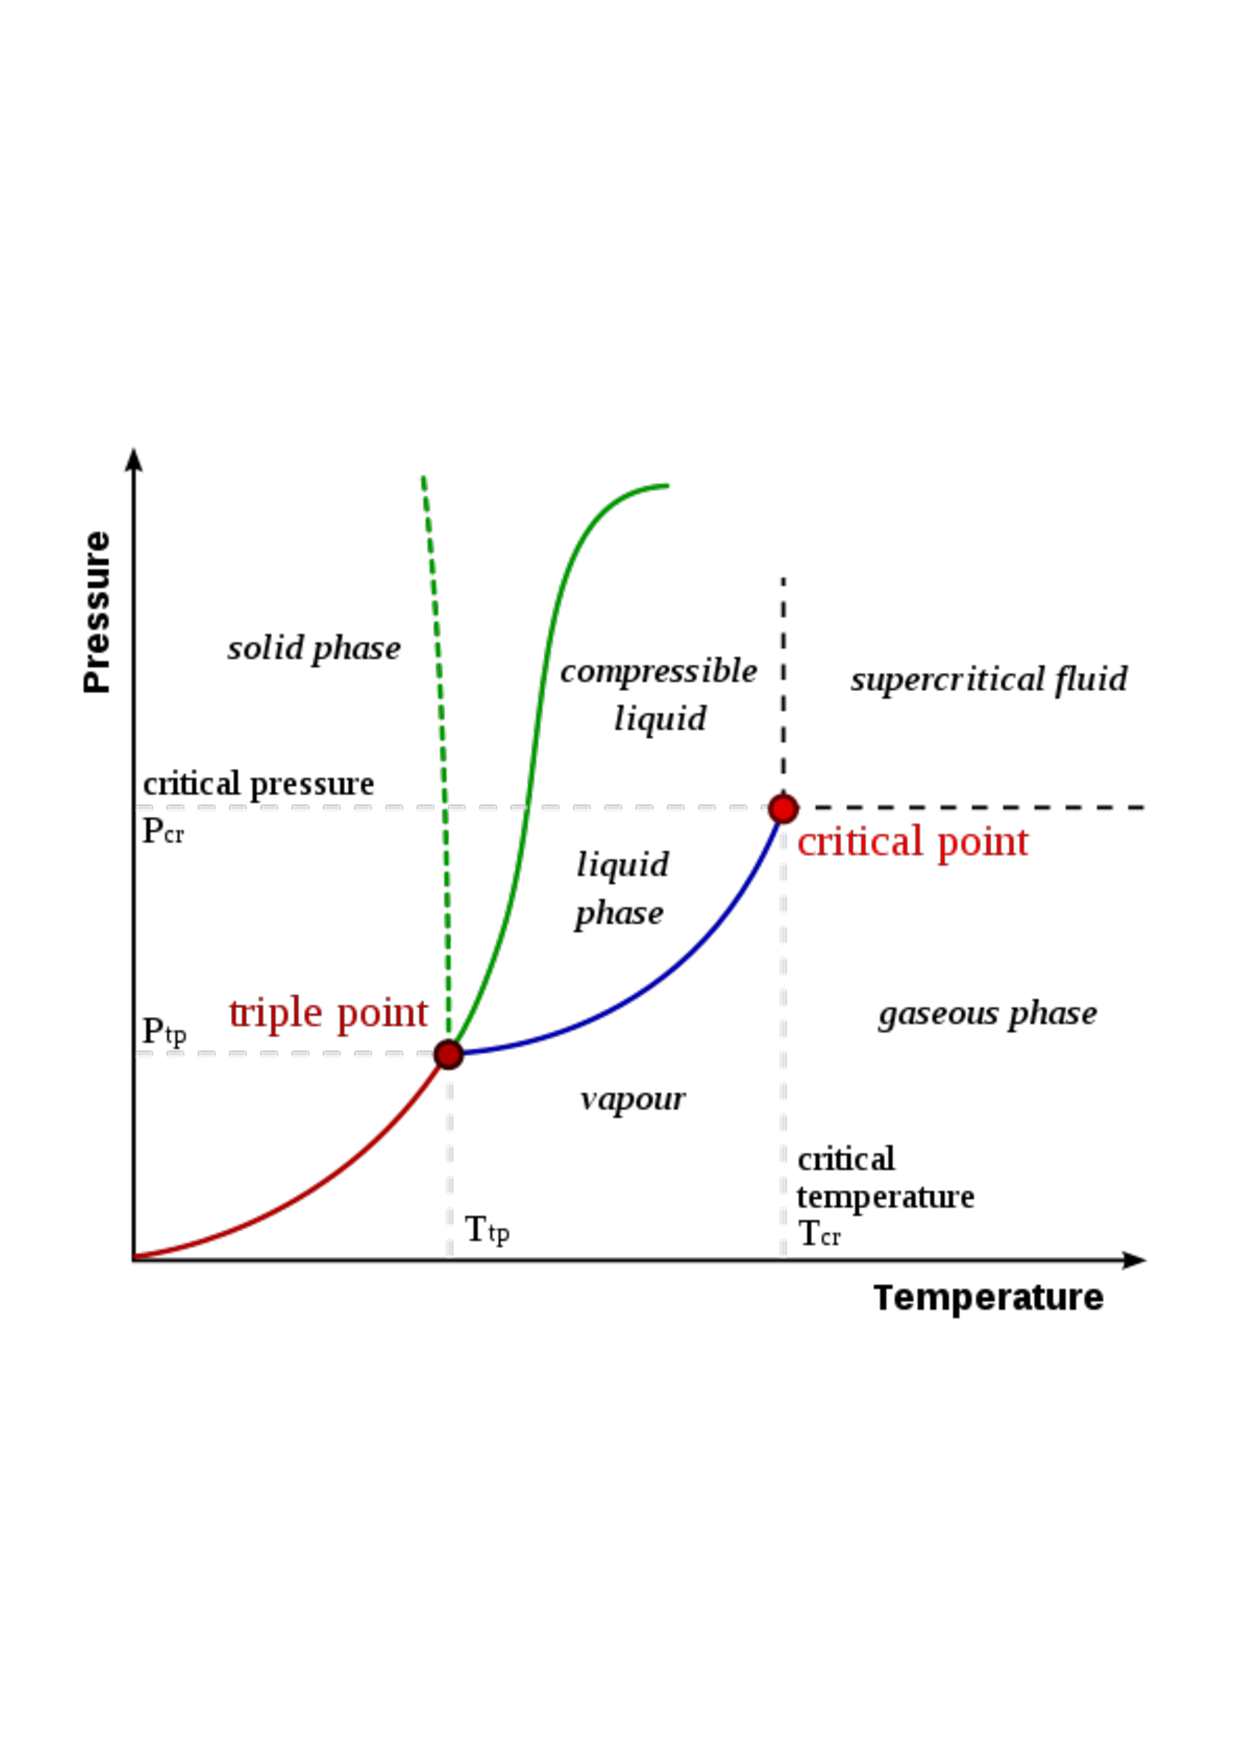
\includegraphics[width=14cm]{pd_water}
\caption{\bf Phase diagram of water, taken from 'wikipedia'. The dashed green line
is the melting-point line of water (negative slope, anomalous). The solid green line is the melting-point line of most other substances (positive slope, normal).}
%\label{}
\end{center}
\end{figure}


For water:
$T_{tp}=273,16000 K (0,01000 C)$, $p_{tp}=611,657 Pa$.
$T_{c} = 647.096 K$, $p_{c} = 22.064 MPa$ and $\rho_{c} = 356 kg/m^{3}$.

Names of phase transitions
\begin{itemize}
	\item solid $\leftrightarrow$ liquid: melting, freezing 
 	\item liquid $\leftrightarrow$ gas:  vaporization, condensation
 	\item solid $\leftrightarrow$ gas: sublimation, deposition
\end{itemize}

Anomaly of water: increasing temperature reduces volume and the density increases. By increasing 
pressure, solid water becomes liquid. Hence, the density of solid water (ice) is smaller than that of liquid water. That is the reason why ice floats on water and why  creatures living in water  survive in winter.

Water is a one component liquid, i.e. $\alpha=1$. 

\subsubsection{a) Pure phases (solid,liquid,gas), $\Nphases =1$}

The number of d.o.f. is 
%
\begin{align*}
f = 2 + \alpha -\Nphases  = 2 + 1 - 1 = 2\;,
\end{align*}
%
which means we can vary to state vasriables, here $T$ and $p$, independently.

\subsubsection{b) Two coexisting phases, $\Nphases =2$}
\begin{itemize}
   \item boiling curve (liquid to gas)
 \item condensation curve (gas to liquid)
	\item melting curve (solid to liquid)
 \item solidification curve (liquid to solid)

\item sublimation curve (solid to gas)
\item resublimation curve (gas to solid)
	
\end{itemize}


The number of d.o.f. is 
%
\begin{align*}
f = 2 + 1 - 2 = 1\;,
\end{align*}
%
which means, we have to vary  $T$ and $p$ on a curve, $p(T)$, e.g. melting-point line.



\subsubsection{c) Three coexisting phases, $\Nphases =3$, triple point}

Here $f=0$. There is no degree of freedom. 

It also follows that for a one-component substance there are at most 3 phases, otherwise the
number of d.o.f. would become negative.


\subsection{Clausius-Clapeyron}

As a further application of the previous discussion, we consider the coexistence line between
liquid and gas (Condensation curve) of a one-component system, such as water. 

If we choose $T$ and $P$ as the two independent d.o.f. then according to 
\eq{eq:mu:condition} we have
%
\begin{align}\label{eq:mu:coexist}
\mu_{fl}(T,p) &= \mu_{g}(T,p)\;.
\end{align}
%
This relation allows to determine to condensation curve $p(T)$ on which the fluid and the gas phase coexist. Away from this curve, only one phase exists, namely the one where the chemical potential is smaller. This is due to the Gibbs-Duhem relation for the free Enthalpy
%
\begin{align*}
G(T,p,N) &= \mu N\;.
\end{align*}
% 
In the case of a single phase, the system will minimize the Free Enthalpy $G$. Since $N$ is fixed,
the phase with  the smaller chemical potential has a smaller Free Enthalpy.

The free Enthalpy is related to the free energy $F(T,V,N)$ via a Legendre transformation,
where $V$ is replaced by $p$. We start out with
%
\begin{align*}
\frac{\partial }{\partial V} F(T,V,N)\at_{T,N} &= - p
\end{align*}
%
This relation can be inverted for given $T,N$ and $p$ we obtain
%
\begin{align*}
V &=V(p,T,N)
\end{align*}
%
%
\begin{align}
G(T,p,N) &= F(T,V(p,T,N),N) + p V\;.
\end{align}
%
Then
%
\begin{align*}
dG &= dF +pdV + Vdp\\
&= -SdT -p dV +\mu dN +pdV + Vdp\;.
\end{align*}
%
Hence  we have
%
\begin{align*}
dG &= \mu dN - S dT + V dp\;,
\intertext{or rather}
dG - \mu dN &= - S dT + V dp\;.
\end{align*}
%
On the other hand the Gibbs-Duhem relation yields
%
\begin{align*}
dG &= \mu  dN + N d\mu\Rightarrow dG - \mu dN = N d\mu\;.
\end{align*}
%
Combining the two relation yields
%
\begin{align*}
- S dT + V dp &= N d\mu\;.
\end{align*}
%
This is generally valid and it also applies individually to different phases, which here shall
have the same $T$ and $p$, i.e.
\begin{align*}
- S_{\nu} dT + V_{\nu} dp &= N_{\nu} d\mu_{\nu}\notag\\
- \frac{S_{\nu}}{N_{\nu}} dT + \frac{V_{\nu}}{N_{\nu}} dp &=  d\mu_{\nu}\;.
\end{align*}
We introduce entropy and volume per particle
%
\begin{align}\label{eq:}
s_{\nu} &= \frac{S_{\nu}}{N_{\nu}}\\
v_{\nu} &= \frac{V_{\nu}}{N_{\nu}}\;,
\end{align}
%
and obtain
%
\begin{align}\label{eq:dmu:nu}
- s_{\nu}  dT + v_{\nu} dp &=  d\mu_{\nu}\;.
\end{align}
%
%
%
Now we consider changes $dp,dT$ along the coexistence line.
There we have due to \eq{eq:mu:coexist}
%
\begin{align*}
d\mu_{fl}(T,p) &= d\mu_{g}(T,p)\;.
\end{align*}
%
Along with \eq{eq:dmu:nu} we obtain
\begin{align*}
- s_{fl}  dT + v_{fl} dp &= - s_{g}  dT + v_{g} dp \\
\frac{dp}{dT} &= \frac{s_{g}-s_{fl}}{v_{g}-v_{fl}} = \frac{\Delta s}{\Delta v}\;.
\end{align*}
Finally, we define the molar vaporation enthalpy
%
\begin{align*}
q &= T\big( s_{g}-s_{fl} \big)
\end{align*}
%
and find the
\tboxit{Clausius-Clapeyron relation}{
%
\begin{align}\label{eq:}
\frac{dp}{dT}&= \frac{q}{T\big( v_{g}-v_{fl} \big)}\;.
\end{align}
%
}
In the derivation of the Clausius-Clapeyron relation we have assumed that $ S_{g}\ne S_{fl}$
and $V_{g}\ne V_{fl}$, which means, although 
%
\begin{align*}
\mu_{g}(T,p) &=\mu_{fl}(T,p) 
\end{align*}
%
that
%
\begin{align*}
\frac{\partial \mu_{g}}{\partial T}\at_{p} &\ne \frac{\partial \mu_{fl}}{\partial T}\at_{p}\\
\frac{\partial \mu_{g}}{\partial p}\at_{T} &\ne \frac{\partial \mu_{fl}}{\partial p}\at_{T}\;.
\end{align*}
%
Such a phase transition is a first order phase transition.

The Clausius-Clapeyron relation is only valid for first order phase transitions.

\subsection{Real gases (van der Waals equation)}
In an  earlier chapter we have discussed the ideal gas and its equation of state

%
\begin{align*}
p V &= N k_{B} T\;.
\end{align*}
%
We also introduced finite eigen-volumes of the moelcules and obtained
%
\begin{align*}
p \big(V- V_{0}\big) &= N k_{B} T\;.
\end{align*}
%
Finally, we also want to include the intermolecular forces. For molecules in the bulk of the 
material, these forces vanish on average, as they act with equal strength in opposite directions.
This is not the case in the surface layer, where the partners outside the surface are missing.
This results in an effective force, pulling the molecules  in the surface layer into the bulk. I.e.
the intermolecular forces act at the surface like an additional pressure (internal pressure).
It has the form 
%
\begin{align*}
a \frac{N^{2}}{V^{2}}
\end{align*}
%
resulting in 
\tboxitp{van der Waals equation}{extensive form}{
%
\begin{align}\label{eq:vdW:ext}
\bigg( p + a' \frac{N^{2}}{V^{2}} \bigg)\bigg(V - \overbrace{N b'}^{V_{0}} \bigg) &= N k_{B} T\;.
\end{align}
%
}
It can also be expressed in terms of molar volume $v$, pressure and temperature, i.e.
the intensive form 
\tboxitp{van der Waals equation}{intensive representation}{
%
\begin{align}\label{eq:vdW:int}
\bigg( p + \frac{a'}{v^{2}} \bigg)\bigg(v - b' \bigg) &= k_{B} T\;.
\end{align}
%
}
Here, $b'$ is the eigen-volume of one molecule.

We multiply \eq{eq:vdW:int} by $v^{2}$ and find that it becomes a cubic equation in $v$
%
\begin{align*}
\bigg( p v^{2}+ a' \bigg)\bigg(v -  b' \bigg) - k_{B} T v^{2}&= 0\\
p v^{3} + a' v   -  b' p v^{2} - a' b' - k_{B} T v^{2}&= 0\;.
\end{align*}
%
Next we introduce suitable units $p_{cr},v_{cr},T_{cr}$ and the corresponding dimensionless 
quantities $\pi,\nu,t$ via
%
\begin{align*}
p &=\pi p_{cr}\\
v &=\nu v_{cr}\\
T &= t T_{cr}\;,
\end{align*}
%
resulting in 
%
\begin{align*}
\pi \nu^{3} + \frac{a' v_{cr}}{p_{cr} v_{cr}^{3} } \nu -\frac{b' p_{cr}  v_{cr}^{2}}{p_{cr} v_{cr}^{3} } \pi \nu^{2}
-\frac{a'b'}{p_{cr} v_{cr}^{3} } - \frac{k_{B}T_{cr} v_{cr}^{2}}{p_{cr} v_{cr}^{3} } t \nu^{2}&=0 \\
\pi \nu^{3} + \underbrace{
\bigg(\frac{a' }{p_{cr} v_{cr}^{2} }\bigg) 
}_{\color{blue} = T_{1}}\nu
 -\underbrace{
\bigg(\frac{b'  }{ v_{cr} }\bigg) 
}_{\color{blue} = T_{2}}\pi \nu^{2}
-\underbrace{
\bigg(\frac{a'b'}{p_{cr} v_{cr}^{3} }\bigg)
}_{\color{blue} = T_{3}} - 
\bigg(\frac{k_{B}T_{cr} }{p_{cr} v_{cr} } \bigg)
t \nu^{2}&=0 \\
\pi \nu^{3} + T_{1}\nu - T_{2} \pi \nu^{2}
-T_{3} - 
\underbrace{
\bigg(\frac{k_{B}T_{cr} }{p_{cr} v_{cr} } \bigg)
}_{\color{blue} = T_{4}} t \nu^{2}&=0 \;.
\end{align*}
%
Now we have the freedom to choose the parameters $p_{cr}$, $v_{cr}$, and $T_{cr}$ suitably.
We use
%
\begin{align}
T_{_{2}} &=\bigg(\frac{b'  }{ v_{cr} }\bigg)= \frac{1}{3}\\
T_{3}&= \bigg(\frac{a'b'}{p_{cr} v_{cr}^{3} }\bigg) =1\\
T_{4}&=\bigg(\frac{k_{B}T_{cr} }{p_{cr} v_{cr} } \bigg)= \frac{8}{3}
\end{align}
%
then
\tboxitp{Critical values}{van der Waals}{
\begin{align}\label{def:critical:values}
v_{cr} &= 3 b'\\
\Rightarrow\qquad p_{cr}&= \frac{a'b'}{ v_{cr}^{3} } = \frac{a'}{27b'^{2}}\\
\Rightarrow\qquad T_{1}&= \frac{a'}{p_{cr} v_{cr}^{2}} = \frac{a'}{\frac{a'}{27 b'^{2}}9 b'^{2}} = 3\\
k_{B}T_{cr} &= \frac{8}{3} p_{cr} v_{cr} =\frac{8}{3} \frac{a'}{27 b'^{2}}\;3 b'
=\frac{8 a'}{27 b'}\;.
\end{align}}
%
So we have
%
\begin{align}\label{eq:auxaux}
\pi \nu^{3} + 3 \nu -  \frac{\pi \nu^{2}}{3} - 1 &= \frac{8}{3}t \nu^{2}\\
\bigg( \pi + \frac{3}{\nu^{2}} \bigg)\bigg( \nu - \frac{1}{3} \bigg) &=\frac{8}{3} t\;.
\end{align}
%
Solving for $\pi$ yields
%
\begin{align*}
\pi &= \frac{8t}{3 \nu-1 } - \frac{3}{\nu^{2}}
\end{align*}
%
The term $(3\nu-1)$ originated from $V-V_{0}$, and therefore it is always positive,
as the total volume has to be greater than the eigen volume. 

If we plot $\pi(\nu)$ for fixed $t$ (isotherm) then we find different behaviour for $t<1$, $t=1$ and $t>1$.
%
\begin{figure}[htbp]
\begin{center}
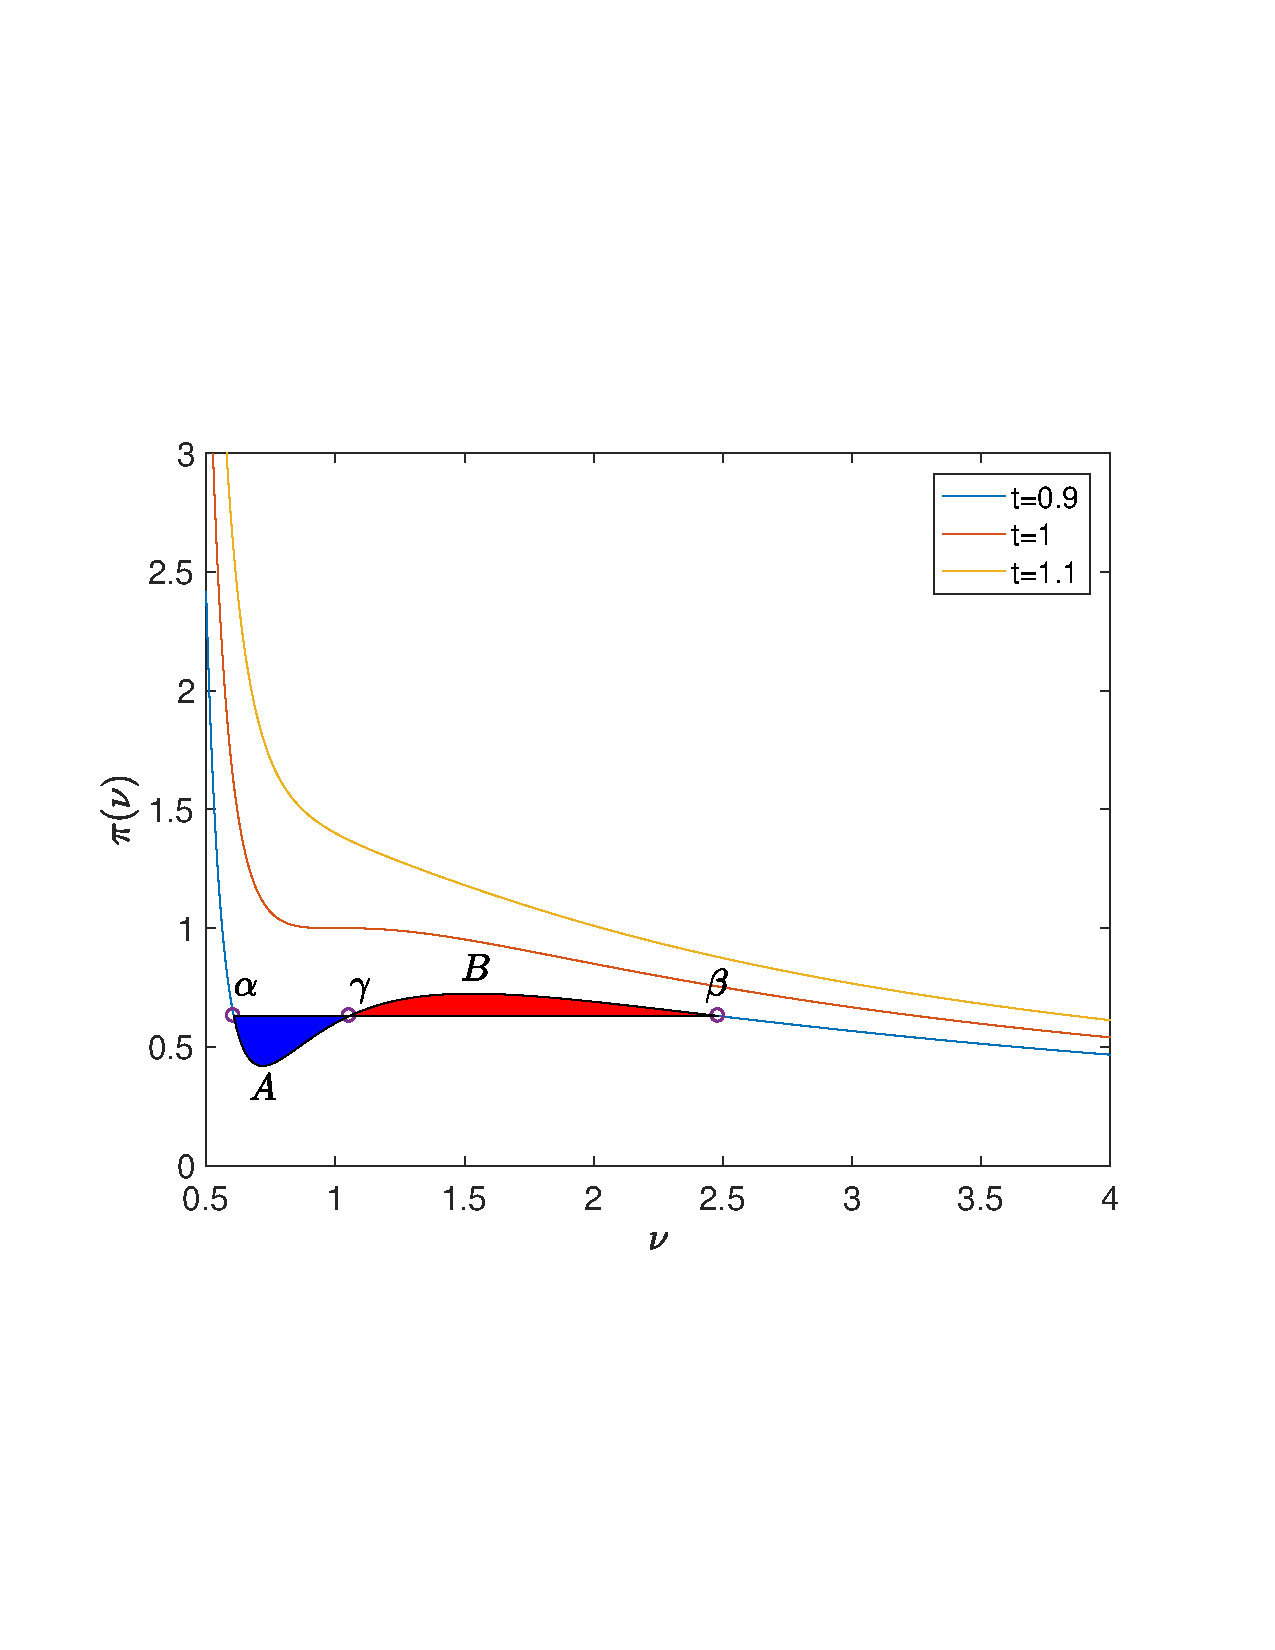
\includegraphics[width=10cm]{Maxwell}
\caption{\bf Maxwell construction.}
\label{fig:Maxwell}
\end{center}
\end{figure}
%
\begin{itemize}
\item For $t<1$ the curve has a minimium and a maximum in the physical interval $\nu>1/3$.
\item For $t=1$ minimum and maximum coincide at $\nu=1$, with $\pi(\nu=1)=1$.
 \item For $t>1$ the curve is monotonically decreasing in the physical interval.
\end{itemize}
We will see soon that there is a phase transition if the curve has a maximum and a minimum.
 If it is monotonically decreasing, there is no phase transition. Hence, the parameters
 $p_{cr}$,  $v_{cr}$, and  $T_{cr}$ represent the  critical point.
 
 
Inserting the critical values into the van-der-Waals equation of state in form of the following ratio
then we obtain
%
\begin{align}\label{def:Z:cr}
Z:=\frac{p_{cr} v_{cr}}{k_{B} T_{cr}} &=  \frac{\frac{a'}{27 b'^{2}}3 b'}{\frac{8 a'}{27 b'}} =
\frac{3}{8}\;.
\end{align}
%
Experimentally one finds for all real gases at the critical point $Z<3/8$, while the ideal gas yields $Z=1$. In this respect the van der Waals model is clearly better.
Alternatively, \eq{def:Z:cr} can be written with $\rho_{c}=1/v_{cr}$ as
%
\begin{align}\label{eq:p:cr}
p_{cr} &=\frac{3}{8} k_{B} T_{cr} \rho_{cr}\;.
\end{align}
%

\subsection{Maxwell-Construction}

We have just seen that the equation of state for the van der Walls model reads in dimensionless units
%
\begin{align*}
\bigg( \pi - \frac{3}{\nu^{2}} \bigg)\bigg(\nu  -\frac{1}{3}\bigg) &=\frac{8}{3} t\;,
\end{align*}
%
and that  $t<1$ there   are regions in the $\pi-\nu$-diagramm where the isotherm compressiblility
%
\begin{align}\label{eq:}
\kappa_{T}&= - \frac{1}{V} \bigg(  \frac{\partial V}{\partial p}\at_{T}\bigg)
= - \frac{1}{p_{cr} \nu} \bigg(  \frac{\partial \nu}{\partial \pi}\at_{T}\bigg) <0
\end{align}
%
becomes negative. This implies that the system is mechanically unstable, it would shrink by itself.

\newpage 

\blue{The reason is  that the van der Waals model describes a single phase of a one-component system.}
It is applicable  in the pure gas or  liquid phase (grey shaded areas in the figure),
but in between there is a phase transition, where two phases coexist, which cannot be described by the van-der-Waals equation.
%
\begin{figure}[htbp]
\begin{center}
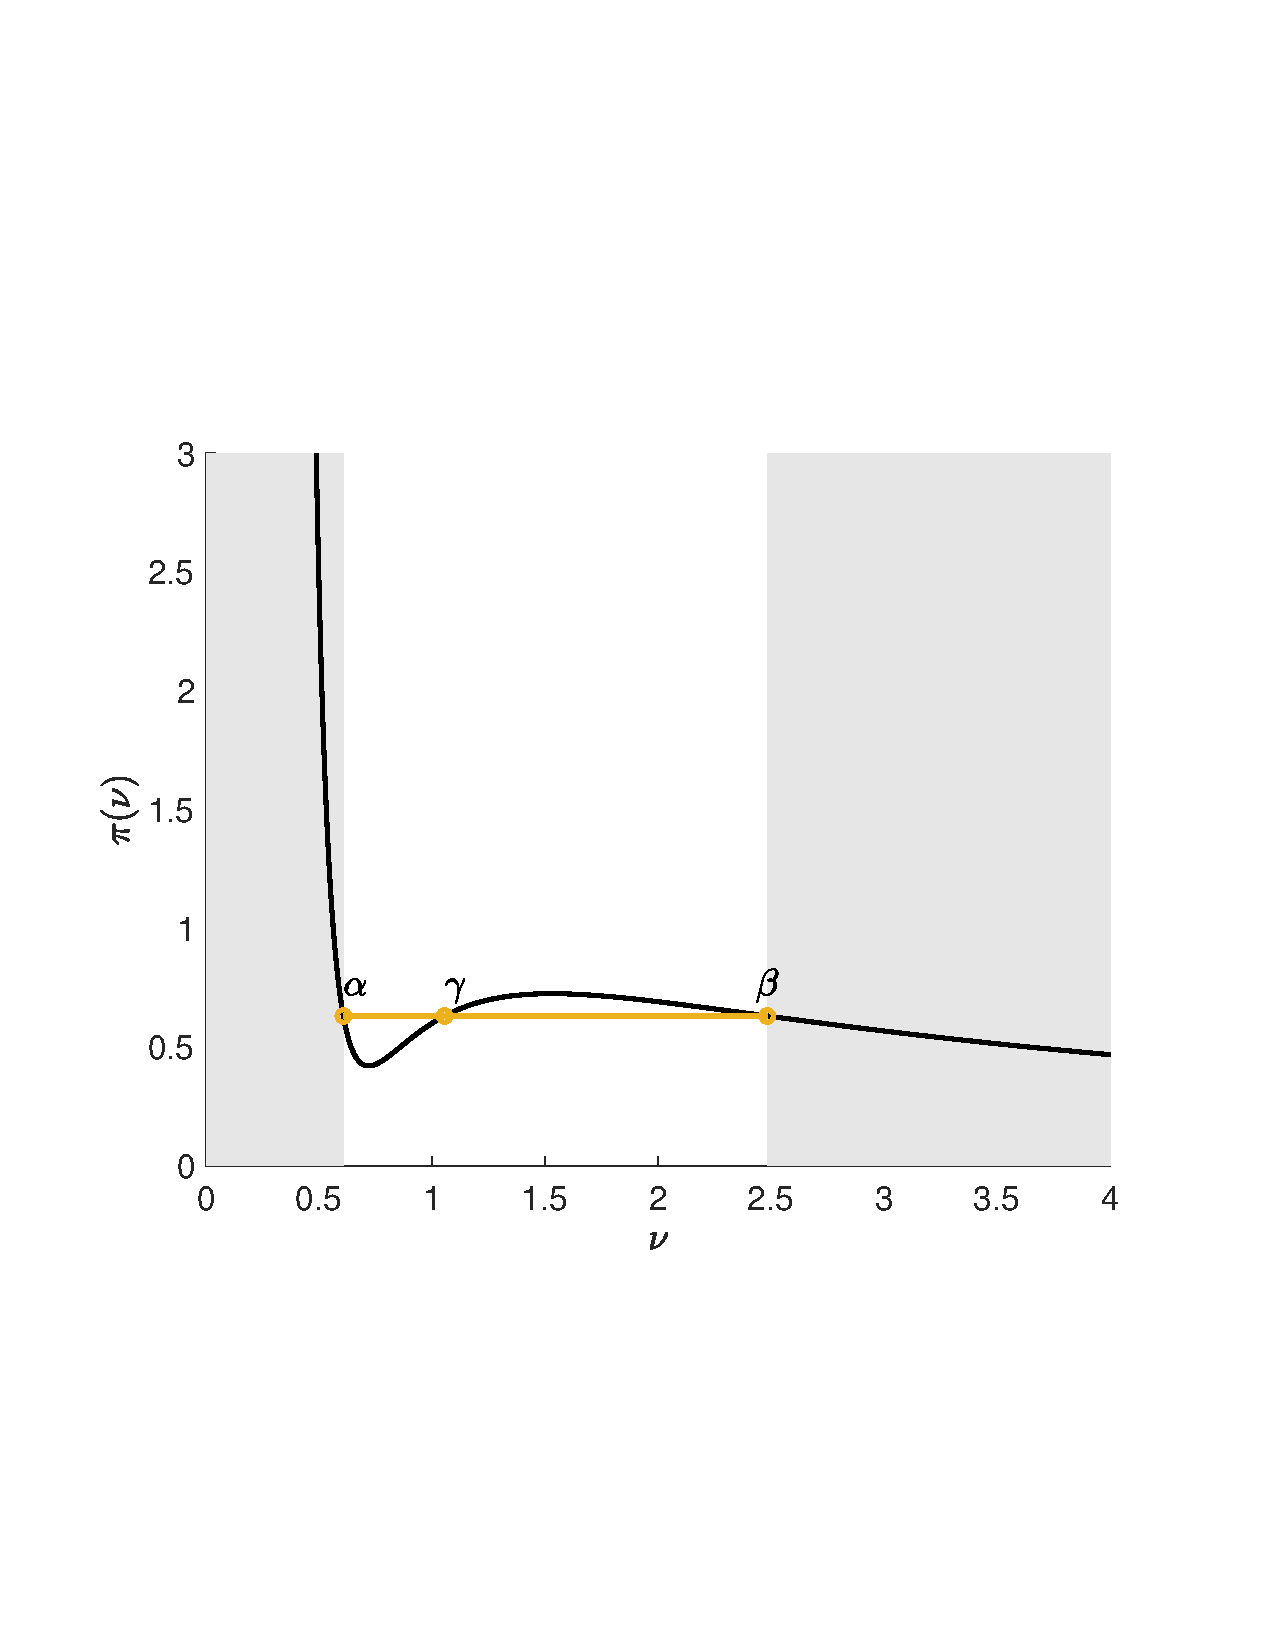
\includegraphics[width=8cm]{Maxwell_new}
\caption{\bf Maxwell construction.}
\label{fig:Maxwell}
\end{center}
\end{figure}
%


What happens in reality is the following. We have seen before that generally on the coexistence 
line between liquid and gas, the number of d.o.f. is merely 1 and it is described by $p=p(T)$.
On isotherms, $T$ is also fixed and therefore $p$ is fixed as well.

%
\nboxit{blue}{All isotherms for ($T<T_{c}$) in the two-phase region have to be horizontal lines in the pV-diagram. (See golden line in the figure )} 

We denote the pressure on the coexistence line between the points $\alpha$ and $\beta$ in the 
$\pi-\nu-$ diagram by $p_{\alpha\beta}$.

In the pure phases of a one-component system we have only two d.o.f., e.g.
$p$ and $T$.
Since the van-der-Waals model is still valid in the pure phase regions (grey shaded),
we have the condition (\eq{eq:mu:coexist})
%
\begin{align*}
\mu_{fl}(T,p) &= \mu_{g}(T,p)\;.
\end{align*}
%
Hence for the isotherm compression, discussed before, the pressure  ($p_{\alpha\beta}$) when reducing the volume in the two-phase region, does not change and we have
%
\begin{align*}
\mu_{fl}(T,p_{\alpha\beta}) &=\mu_{g}(T,p_{\alpha\beta})\;.
\end{align*}
%
In addition, at the points $\alpha$ and $\beta$, we have pure phases and therefore $N_{\alpha}=N$ and $N_{\beta}=N$ and consequently at the end points of the horizontal line we have
%
\begin{align*}
\mu_{fl}(T,P_{\alpha\beta}) N_{\alpha} &=\mu_{g}(T,P_{\alpha\beta}) N_{\beta}
\end{align*}
%
Then the Gibbs-Duhem relation ($G=\mu N$)  yields for these points
%
\begin{align*}
G_{\alpha} &= G_{\beta}\\
F_{\alpha} + p_{\alpha}V_{\alpha} &=F_{\beta} + p_{\beta} V_{\beta} 
\end{align*}
%
from which we conclude
%
\begin{align}\label{eq:DF:DV}
F_{\alpha}-F_{\beta} &= -p_{\alpha\beta}(V_{\alpha}-V_{\beta})\;.
\end{align}
%
This is the result for the end points of the coexistence line, where we have exploited some of the features of the  two phase region in between, for which we have used $\pi(\nu) = p_{\alpha\beta}$, independent of volume $\nu$.
Alternatively, if we stick to one phase then the van-der-Waals equation determines the pressure curve, the one given in figure \ref{fig:Maxwell} with the wavy look.
In that case, the differential of the free energy is, since $N$ is fixed and $T$ is fixed (isotherm),
%
\begin{align*}
dF &= S dT - pdV +\mu dN = -pdV\;,
\end{align*}
%
and the integral yields
%
\begin{align*}
F_{\alpha}-F_{\beta} &= \int_{{\beta}}^{\alpha} dF =
- \int_{V_{\beta}}^{V_{\alpha}} p(T,V',N)  dV' \;.
\end{align*}
%

%
\begin{align}\label{eq:DF:DV:2}
F_{\alpha}-F_{\beta} &= \int_{V_{\alpha}}^{V_{\beta}} p(T,V',N)  dV' 
\end{align}
%
By combining \eq{eq:DF:DV} and \eq{eq:DF:DV:2} we find

%
\begin{align}\label{eq:aux:vdW}
 \int_{V_{\alpha}}^{V_{\beta}} p(T,V',N)  dV' &=
 p_{\alpha\beta}\;(V_{\beta}-V_{\alpha})
\end{align}
%
I.e., the area under the vdW curve $p(t,V,N)$ as function of volume in the interval  $(V_{\alpha},V_{\beta})$
has to be the same as the area under the constant  $p(V)=p_{\alpha\beta}$ curve in the two-phase region. Consequently, the subareas $A$ and $B$ have to be same.
This tells us how to determine the points $\alpha$ and $\beta$.

Finally, we will show that the pure phase is unstable w.r.t. to the mixed phase. To this end we compare two states with the same $T$ and $V$ but different pressures $p_{\alpha\beta}$
and the vdW pressure $p(T,V,N)$. Since $T$ and $V$ is fixed, we have to compare the free energies.

In the pure phase we compute the free energy for a given $V$ in the interval $(V_{\alpha},V_{\beta})$. To this end we use $dF=-pdV$ and integrate from $V_{\alpha}$ to $V$
%
\begin{align}\label{eq:F:vdW}
F_{vdW}(V,T) &= F_{\alpha} - \int_{V_{\alpha}}^{V} p(V',T) dV'\;.
\end{align}
%



In the two-phase region the free energy is the linear combination of the free energy of the two phases according to their relative size, (extensive quantities!) i.e. 
%
\begin{align}\label{eq:}
F_{mp} &=  c_{fl} F_{fl} + c_{g} F_{g}\\
 &=  c_{fl} F_{\alpha} + c_{g} F_{\beta}\;,
\end{align}
%
with $c_{fl}=N_{fl}/N$ and $c_{g}=N_{g}/N$, hence $c_{fl}+c_{g}=1$\;.
Then
\begin{align}
F_{mp} &=  F_{\alpha}+ (c_{fl}-1) F_{\alpha} + c_{g} F_{\beta}\notag\\
 &=  F_{\alpha}- c_{g} F_{\alpha} + c_{g} F_{\beta}\notag\\
F_{mp}  &=  F_{\alpha}+  c_{g} \big(F_{\beta}-F_{\alpha}\big)\label{eq:F:mp:a}\;.
\end{align}
%
Finally, we want  to express $c_{g}$ in terms of volume. The total volume is split accordingly,
%
\begin{align*}
V &= c_{fl} V_{fl} + c_{g} V_{g} = (1-c_{g}) V_{\alpha} + c_{g} V_{\beta} \\
V-V_{\alpha} &= c_{g} \big(V_{\beta}-V_{\alpha}  \big)\\
\end{align*}
%
and we obtain the relative portions of the phases
%
\begin{subequations}\label{eq:rel:port:phase}
\begin{align}
c_{g} &= \frac{V-V_{\alpha} }{V_{\beta}-V_{\alpha} }\\
c_{fl} &=\frac{V_{\beta}-V }{V_{\beta}-V_{\alpha} }\;.
\end{align}
\end{subequations}


%
We then have
%
\begin{align}\label{eq:F:mp:a}
F_{mp} &= 
 F_{\alpha} + \frac{V-V_{\alpha}}{V_{\beta}-V_{\alpha}} \big(F_{\beta}-F_{\alpha}\big)\;.
\end{align}
%
Here we can also use \eq{eq:DF:DV} resulting in
\begin{align}
F_{mp} &= 
 F_{\alpha}-p_{\alpha\beta} \frac{V-V_{\alpha}}{V_{\beta}-V_{\alpha}} \big(V_{\beta}-V_{\alpha}\big)
 =
 F_{\alpha}+p_{\alpha\beta} \big(V-V_{\alpha}\big)
\label{eq:F:mp}
\end{align}
The difference of the free energies is according to \eq{eq:F:vdW} and \eq{eq:F:mp}


%
\begin{align*}
F_{vdW}(V,T) - F_{mp}(V,T) &= 
p_{\alpha\beta} \big(V-V_{\alpha}\big) 
- \int_{V_{\alpha}}^{V} p(V',T) dV'  \ge 0 \;.
\end{align*}
%
The reason can be seen in \fig{fig:Maxwell}. As long as $V\in(V_{\alpha},V_{\gamma})$
it is obvious that the integral over $p(V',T)$ is smaller than the area of the rectangle formed
obtained if $p$ is replaced by $p_{\alpha\beta}$. For $V> V_{\gamma}$ we can modify the equation as follows
\begin{align*}
F_{vdW}(V,T) &- F_{mp}(V,T)  \\
&=p_{\alpha\beta} \big(V_{\gamma}-V_{\alpha}\big) +
p_{\alpha\beta} \big(V-V_{\gamma}\big) 
- \bigg( \int_{V_{\alpha}}^{V_{\gamma}} p(V',T) dV'  + \int_{V_{\gamma}}^{V} p(V',T) dV' \bigg)\\
&= \underbrace{
p_{\alpha\beta} \big(V_{\gamma}-V_{\alpha}\big) -\int_{V_{\alpha}}^{V_{\gamma}} 
p(V',T) dV'}_{\color{blue} = A}
-     \int_{V_{\gamma}}^{V} \big(p(V',T)-p_{\alpha\beta}\big) dV'\\
\end{align*}
%
For $V \in (V_{\gamma},V_{\beta})$ the integrand  is positive and 
%
\begin{align*}
\int_{V_{\gamma}}^{V} \big(p(V',T)-p_{\alpha\beta}\big) dV' \le B
\end{align*}
%
since $B$ is the value of the integral over the entire interval $(V_{\gamma},V_{\beta})$.
According to the Maxwell construction $B=A$, hence the integral is less then $A$ so in total we find
\begin{align*}
F_{vdW}(V,T) - F_{mp}(V,T)  &\ge 0\;,
\end{align*}
%
as we have claimed before.

\section{Phasetransitions}

In case of the liquid-gas mixture we have seen that the transition occurs for given $T$ at a fixed pressure $p$, the latter is
%
\begin{align*}
p_{\alpha,\beta}(T):\qquad\text{vapor pressure} 
\end{align*}
%
In the transition region we have a mixture of the liquid and the gas state. The percentage portion is given by \eq{eq:rel:port:phase}.

The supplied heat leads to transformation of a fraction of the  fluid into gas. This process is isothermal, since heat is only used to overcome the binding energy present in the fluid.
Only if the entire  fluid is vaporized, further heat transfer results in a temperature rise.
Heat transfer that occurs at a constant system temperature but changes the state variable is 
called latent heat with respect to the variable.

Such phase transitions, that involve {\em latent heat} are {\em first order phase transitions}.
{\em Latent heat} in contrast to {\em sensible heat} does not lead to a change in temperature.

Only for first order phase transitions, the Clausius-Claperyron equation is applicable, as it 
requires that entropy and volume per particle are different in the two phases.

We recall that 
%
\begin{align}\label{eq:}
S &= -\frac{\partial G}{\partial T}\at_{p}\\
V &= -\frac{\partial G}{\partial p}\at_{T}\;.
\end{align}
%
A characteristic feature of first order phase transition is therefore the \blue{discontinuity of the {\bf first} derivative
of the thermodynamic potential} when crossing the coexistence line in the phase diagram.
Along the line it is continuous.

Next we exploit in addition the following relations 
%
\begin{align}\label{eq:}
S &=-\frac{\partial F}{\partial T}\at_{V}\;,\\
p &=-\frac{\partial F}{\partial V}\at_{T}\;.
\end{align}
%
which allow to compute specific heat and compressibility in term of the free enthalpy or free energy
%
\begin{align}\label{eq}
0\le C_{p}&= T \frac{\partial S}{\partial T}\at_{p} =-T 
\frac{\partial^{2} G}{\partial T^{2}}\at_{p}\;\quad &&\Rightarrow \frac{\partial^{2} G}{\partial T^{2}}\at_{p}\le 0\\
0\le \kappa_{T} &= -\frac{1}{V}\frac{\partial V}{\partial p}\at_{T}  =-\frac{1}{V}\frac{\partial^{2} G}{\partial p^{2}}\at_{T}\;\qquad&&\Rightarrow\frac{\partial^{2} G}{\partial p^{2}}\at_{T}\le 0\\
0\le C_{V}&= T \frac{\partial S}{\partial T}\at_{V} =
-T \frac{\partial^{2} F}{\partial T^{2}}\at_{V}\;\quad &&\Rightarrow \frac{\partial^{2} F}{\partial T^{2}}\at_{V}\le 0\\
0\le \frac{1}{\kappa_{T}} &= -V \frac{\partial p}{\partial V}\at_{T}  
=V \frac{\partial^{2} F}{\partial V^{2}}\at_{T}\;\qquad&&\Rightarrow\frac{\partial^{2} F}{\partial p^{2}}\at_{T}\ge 0\;.
\end{align}
%
Therefore we have
\tboxit{}{
%
\begin{align}\label{eq:}
\frac{\partial^{2} G}{\partial T^{2}}\at_{p}\le 0\;,&&\frac{\partial^{2} G}{\partial p^{2}}\at_{T}&\le 0\\
\frac{\partial^{2} F}{\partial T^{2}}\at_{p}\le 0\;,&&\frac{\partial^{2} F}{\partial V^{2}}\at_{T}&\ge 0\;.
\end{align}}
%
I.e. $G$ is concave in both variables $p$ and $T$. Due to $F=G-pV$, it follows that
$F$ is also concave in $T$, but convex in $p$.

\newpage

\subsection{Free energy versus $V$, for $T$ and $N$ fixed}
Since $F>0$ is convex in $V$ and $\frac{\partial F}{\partial V}=-p<0$, $F(V)$  is a decreasing,   left curving line that is always positive and it is strictly monotonically decreasing, as a zero slope  would mean $p=0$. 

The Legendre transform of the free energy $F(V,T,N)$ (in the variable $V$) is the free enthalpy %
\begin{align*}
G(p,T,N) &= F(V(p),GT,N) + p V \\
&= F(V(p),GT,N) - \pder{ F}{V}{T} V
\end{align*}
%


For $T>T_{c}$ the second derivative $\frac{\partial F^{2}}{\partial V^{2}}=-\frac{\partial p}{\partial V}$ is greater than zero (because $\frac{\partial p}{\partial V}<0$)for all $V$.
For $T<T_{c}$, however, there is an interval $(V_{\alpha},V_{\beta})$ in which $\frac{\partial P}{\partial V}=0$ and hence the second derivative is zero and therefore $F(V)$ is a linear function in $V$. Hence,
%
\begin{align*}
\frac{\partial F}{\partial V}\at_{T} &= -p = const = -p_{\alpha\beta}.
\end{align*}
% 

\begin{figure}[ht]
\begin{center}
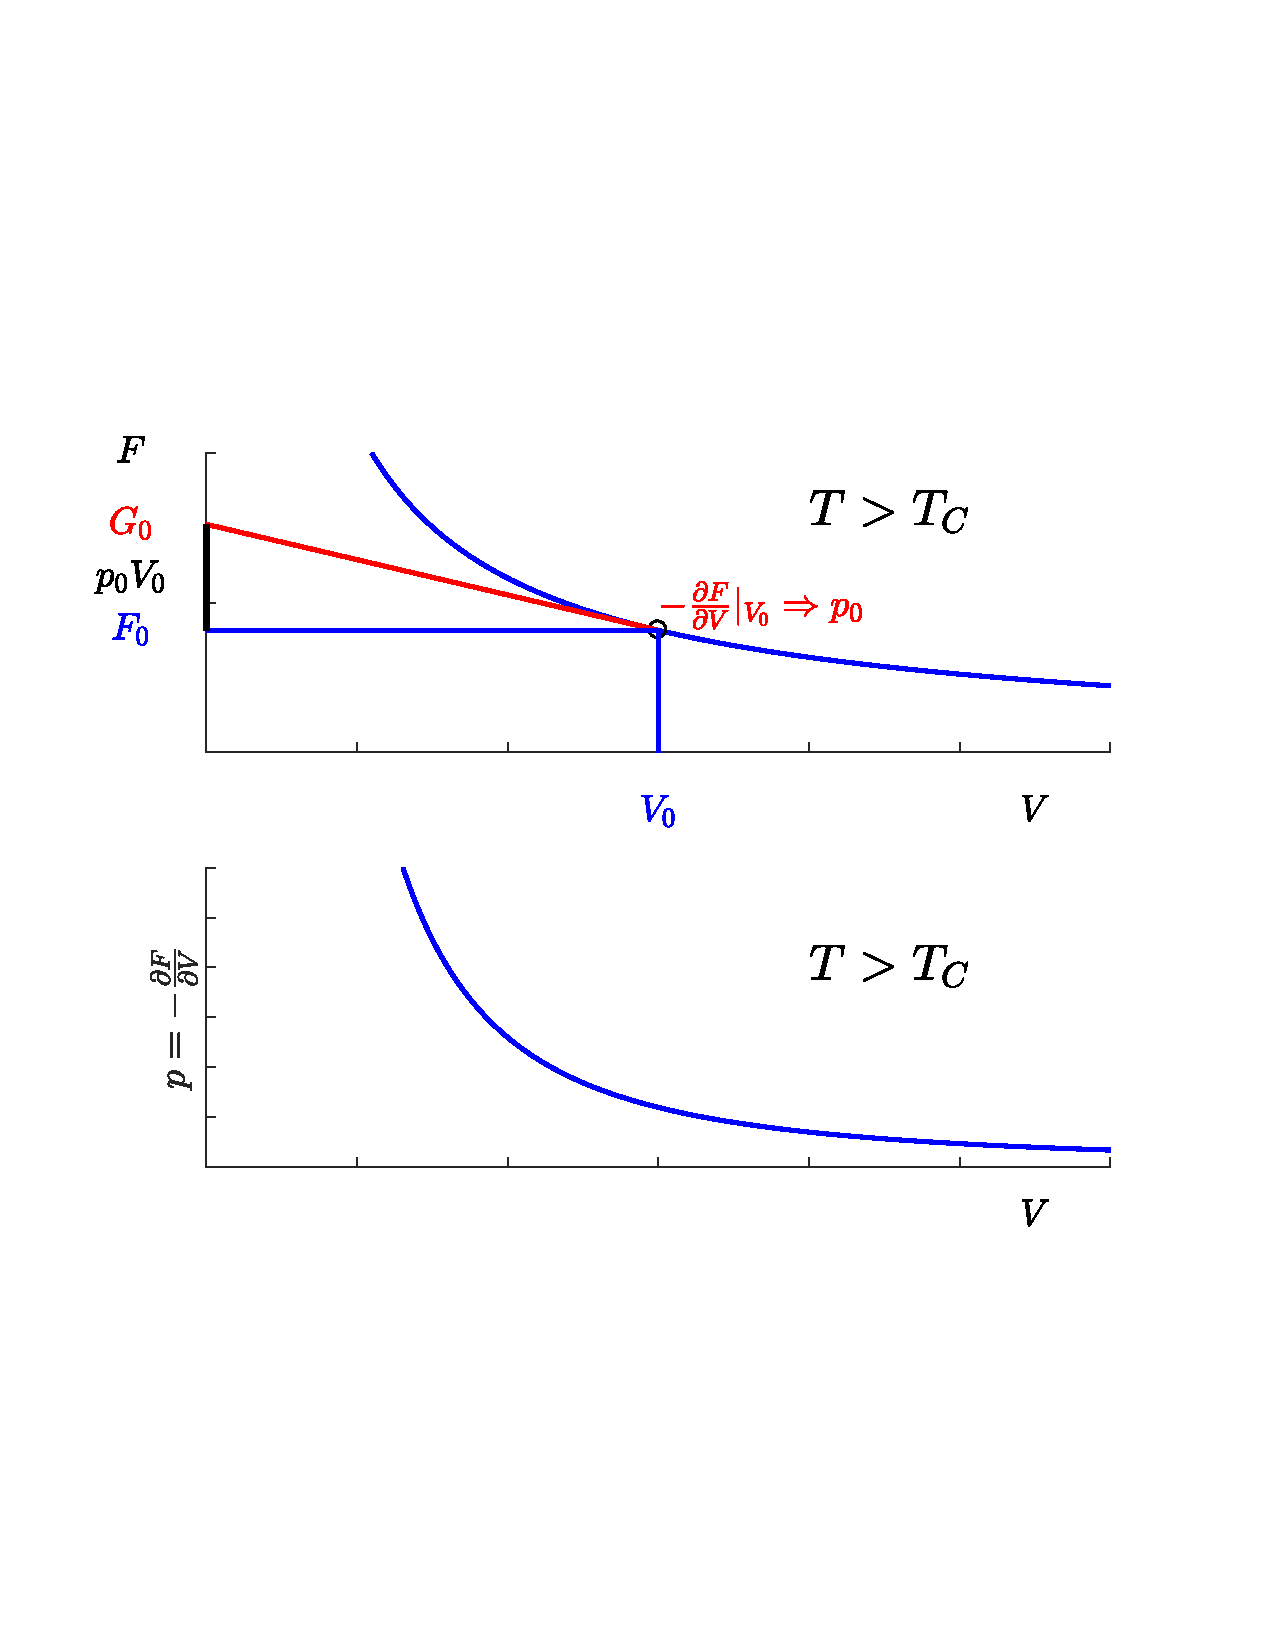
\includegraphics[width=6cm]{convex_above_Tc}
\hfill
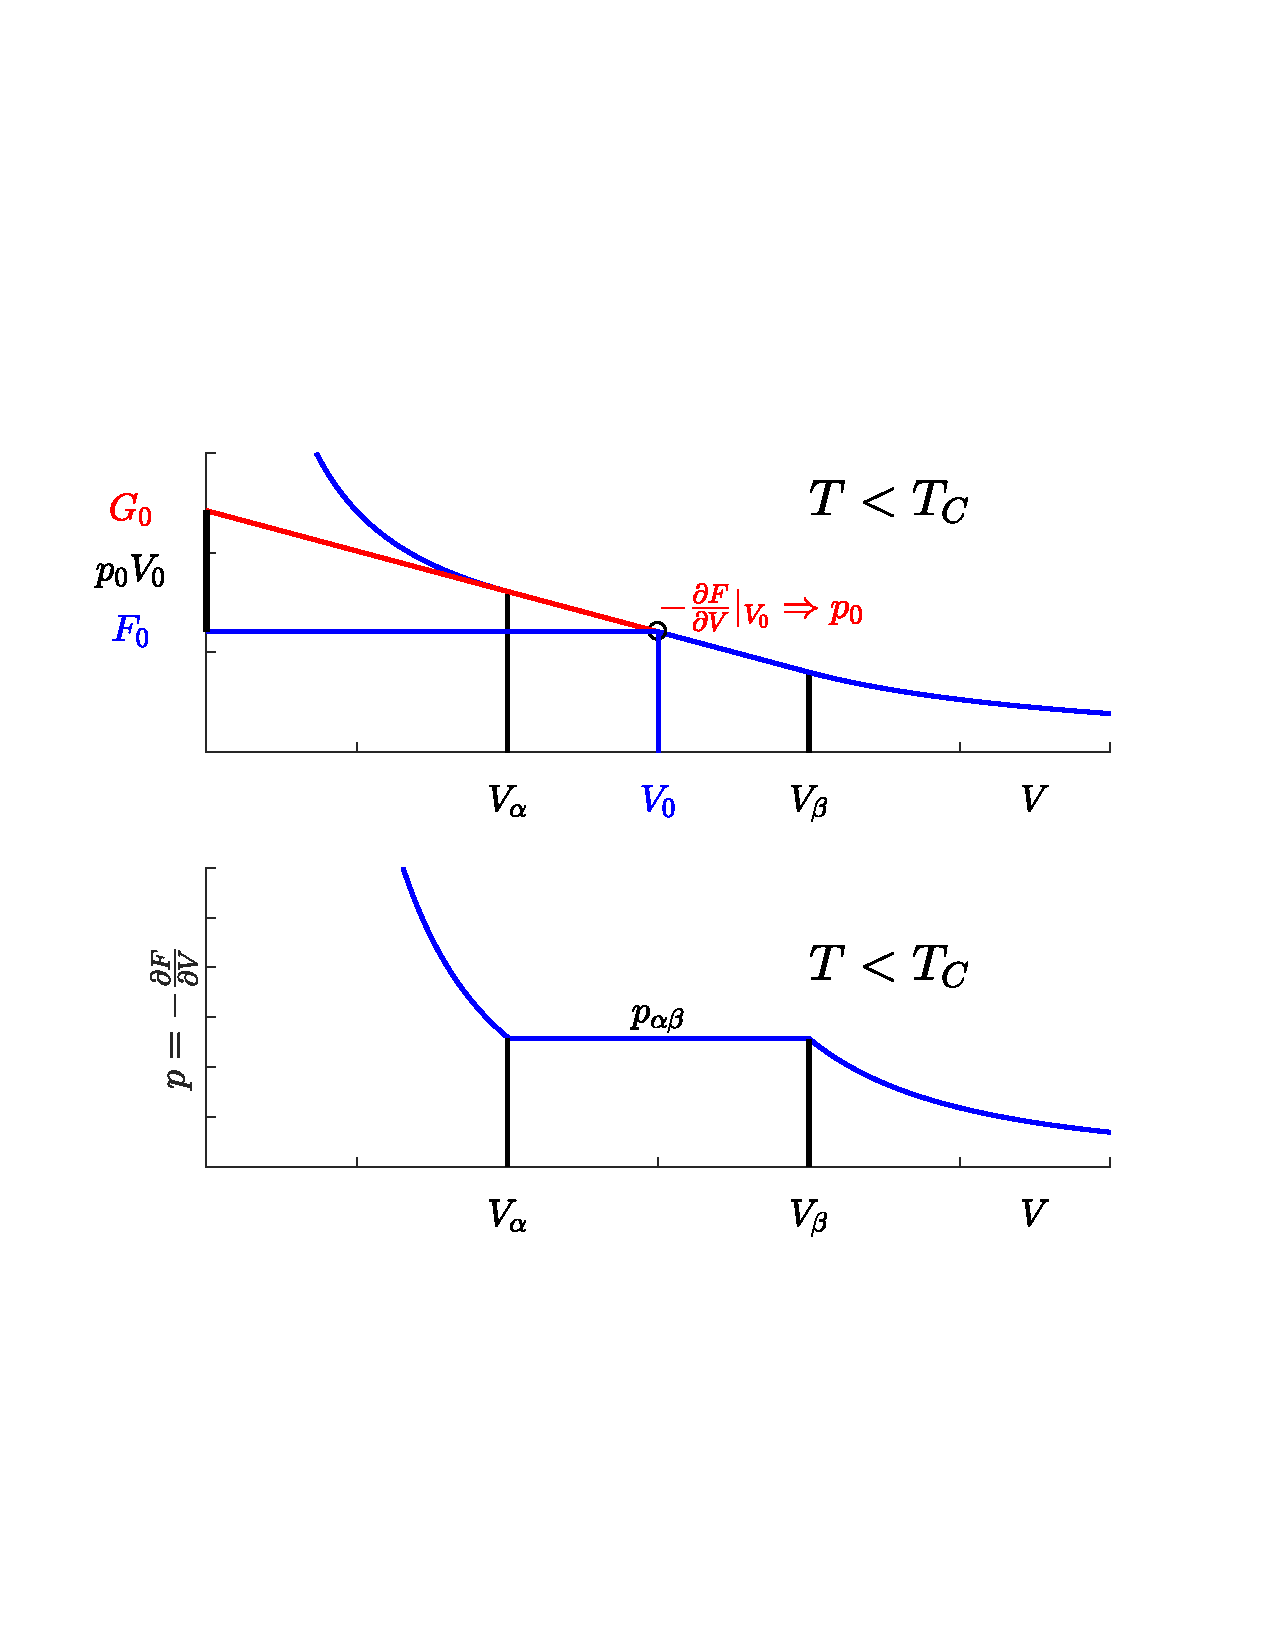
\includegraphics[width=6cm]{convex_below_Tc}
\caption{{\bf Schematic plot of free energy for $T>T_{C}$ (left) and $T<T_{C}$ (right).}}
\end{center}
\end{figure}


%\begin{figure}[ht]
%\begin{center}
%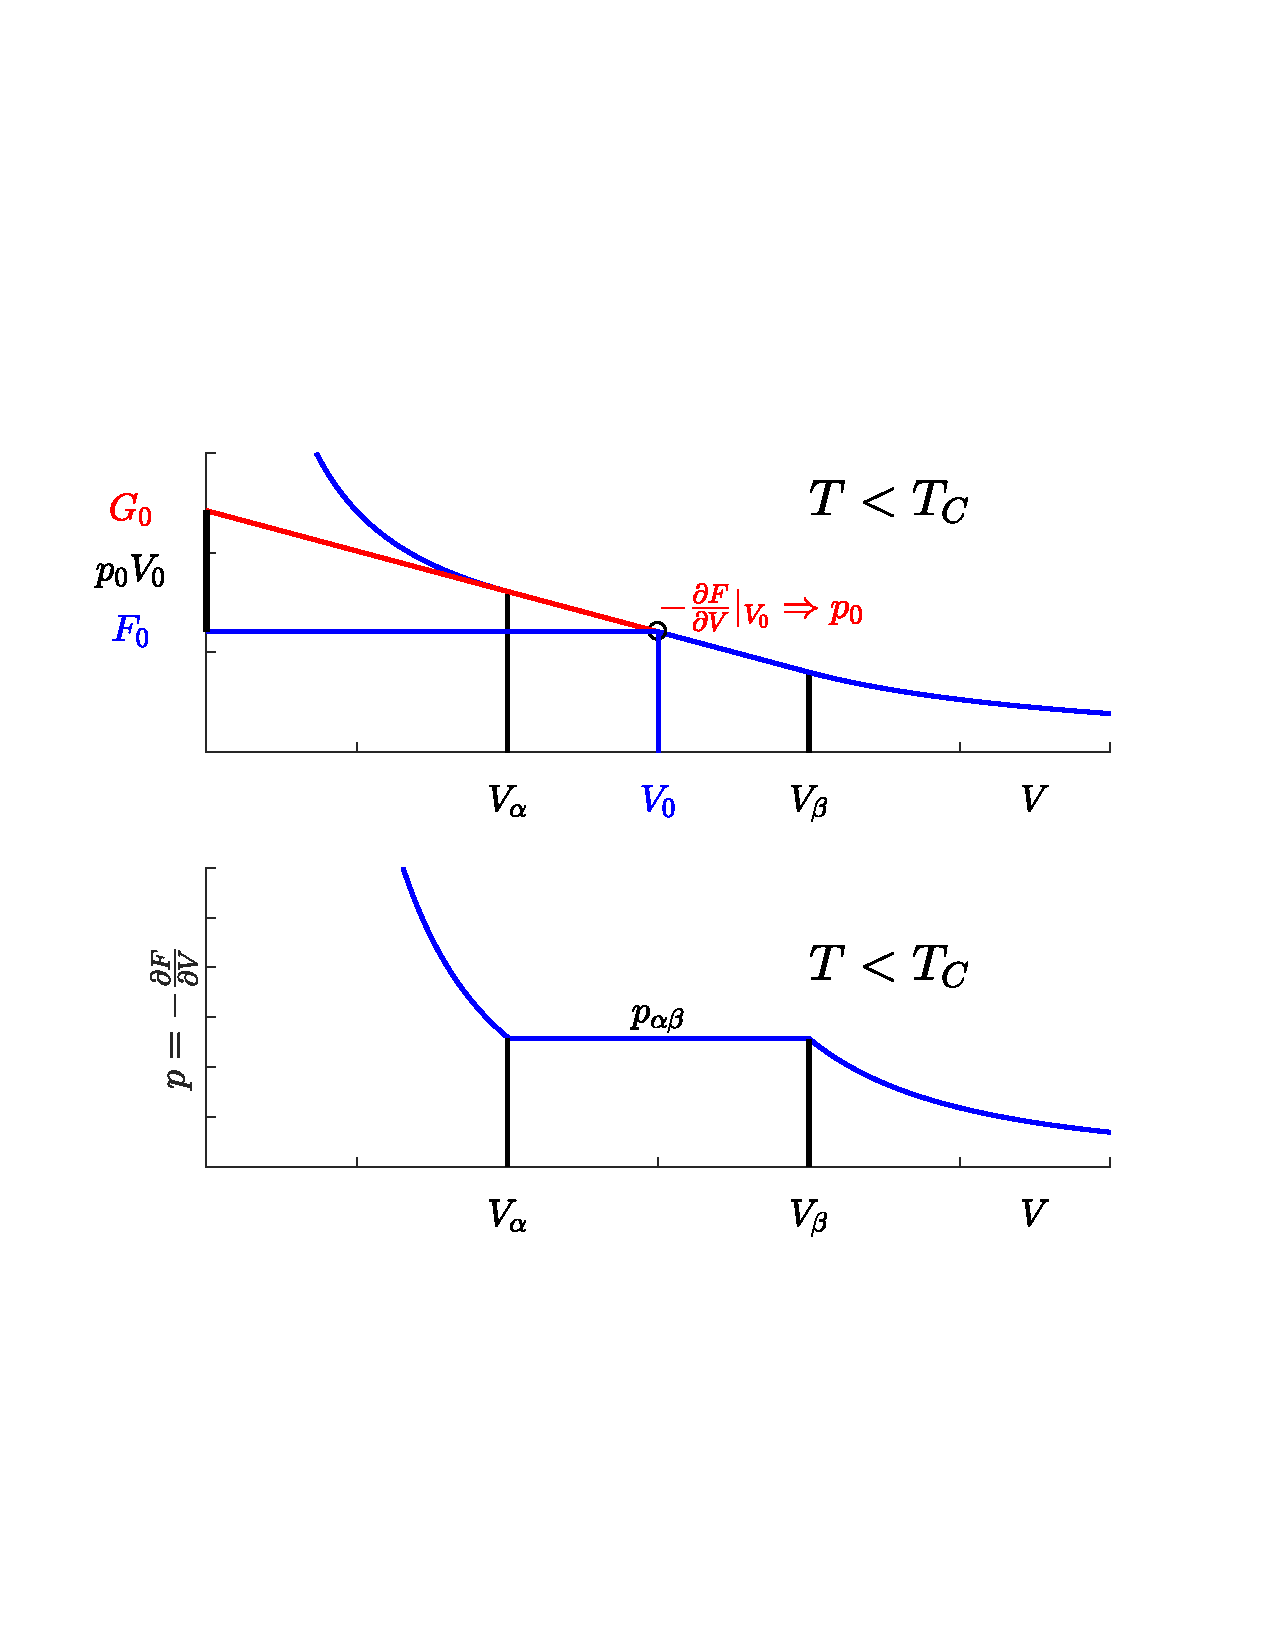
\includegraphics[width=5cm]{convex_below_Tc}
%\caption{{\bf Schematic plot of free energy for $T<T_{c}$.}}
%%\label{}
%\end{center}
%\end{figure}
%

\newpage

\subsection{$F$ and $G$ as function of $T$}

As function of temperature, both $F$ and $G$ behave similarly, since
%
\begin{align*}
-S&=\frac{\partial G}{\partial T}\at_{p}=\frac{\partial F}{\partial T}\at_{V}\;.
\end{align*}
%
At a first order phase transition the entropy $S$ shows a finite jump at $T_{c}$,
which is then associated with 
\tboxit{latent heat}{
%
\begin{align}\label{eq:}
\Delta Q &= T_{\alpha\beta} \Delta S\;.
\end{align}
%
}

$\Delta Q$ is, however not a material constant, it also depends on the state variables e.g.
for the liquid-gas system, $\Delta Q$ depends on pressure. On approaching the \blue{critical point},
$\Delta Q$ vanishes. Therefore, the definition of the order of the phase transition has to refined
\subsection{Ehrenfest classification\label{sec:ehrenfest:classification}}
\tboxit{N-th order phase transition}{
%
\begin{subequations}\label{eq:}
\begin{align}
\frac{\partial^{m} G_{\alpha}}{\partial T^{m}}\at_{p} &=
\frac{\partial^{m} G_{\beta}}{\partial T^{m}}\at_{p}
&&\forall m=1,\ldots n-1\;,\\
\frac{\partial^{m} G_{\alpha}}{\partial p^{m}}\at_{T} &=\frac{\partial^{m}  G_{\beta}}{\partial p^{m}}\at_{T}
&&\forall m=1,\ldots n-1\;.
\intertext{But}
\frac{\partial^{n} G_{\alpha}}{\partial T^{n}}\at_{p} &\ne 
\frac{\partial^{n} G_{\beta}}{\partial T^{n}}\at_{p}\\
\frac{\partial^{n} G_{\alpha}}{\partial p^{n}}\at_{T} &\ne \frac{\partial^{n} G_{\beta}}{\partial p^{n}}\at_{T}\;.
\end{align}
\end{subequations}
}
Of practical importance are first and second order phase transitions. First order phase transitions 
have already been discussed in detail. In the case of a second order phase transition,
we have
\tboxit{Second order phase transition}{
\begin{subequations}\label{eq:}
\begin{align}
G(T,p) &&\text{continuous}\\ 
\frac{\partial G}{\partial T}\at_{p},\frac{\partial G}{\partial p}\at_{T},(\text{i.e. }  
S(T,p), V(T,p)) &&\text{continuous}\\
C_{p}= -T\frac{\partial^{2} G}{\partial T^{2}}\at_{p}\;\quad 
\kappa_{T}= -\frac{1}{V}\frac{\partial^{2} G}{\partial p^{2}}\at_{T}\;\quad
&&\text{discontinous}
\end{align}
\end{subequations}
}

\section{Critical exponents\label{sec:critical:exponents}}
\blue{Second order phase transitions} are of particular interest, as they exhibit universal behaviour close 
to the phase transition. Completely different systems with second order phase transition
show a very similar power law behaviour, which shall be discussed in this section. 
We define 
%
\begin{align*}
\varepsilon &=\frac{T-T_{C}}{T_{C}}\;.
\end{align*}
%
Very often it is observed that in a close vicinity of $T_{c}$, typically
$\abs{\varepsilon} < 10^{-2}$,
%
physical observables $f(T)$ show the following behaviour
%
\begin{align*}
f(\varepsilon) &= a \varepsilon^{\varphi} \big( 1 +  b \varepsilon^{\psi} +\ldots\big)\;\psi>0\;,
\end{align*}
%
here $\varphi$ and $\psi$ are real valued exponents. This behaviour is abbreviated as
%
\begin{align}
f(\varepsilon) &\simeq \varepsilon^{\varphi}\;,
\end{align}
%
One says: $f$ behaves like $\varepsilon^{\varphi}$ and $\varphi$ is called the {\em critical exponent}.
The critical exponent is more generally defined by
%
\begin{align}\label{def:critical:exponent}
\varphi &= \lim_{\varepsilon\to 0} \frac{
\ln \abs{f(\varepsilon)} }{\ln \abs{\varepsilon}}
\end{align}
%
In general, the critical exponent depends on whether we compute it below or above $T_{c}$.
For the \blue{order parameter} it actually makes only sense below  $T_{c}$, as the order parameter
by definition is zero above $T_{c}$.

Of course, different observables may have different critical exponents. The critical exponent for 
one observable, however, is almost universal, it only depends on
\begin{itemize}
	\item spatial dimension
	\item range of the interaction
	\item spin dimensionality.
\end{itemize}

This is the so-called {\em universality hypothesis} of Griffiths.
Te range of the particle interaction is grouped into three classes:
\begin{itemize}
	\item short-range, if the interaction decreases like
%
\begin{align*}
r^{-(d+2+\alpha)}\;;\quad \alpha > 0\;.
\end{align*}
%
Where the details of the interaction are unimportant.
One finds a really universal behaviour.
\item  long-range, if  
%
\begin{align*}
r^{-(d+2+\alpha)}\;;\quad \alpha< \frac{d}{2}-2\quad\text{(always negative)}.
\end{align*}
%  
In this case, the {\em classical theories} apply (Landau Theory, van der Waals model, Weißferromagnet). In this case, however, the critical exponents are independent of the spatial dimension. 
 \item Intermediate range, if 
 %
\begin{align*}
r^{-(d+2+\alpha)}\;;\quad \frac{d}{2}-2 < \alpha < 0\;.
\end{align*}
%
The critical exponents depend on $\alpha$
\end{itemize}


Magnetic systems are typically discussed as interacting spin-systems. As spin-dimension ($n$) we understand the relevant components of the spin vector. Ising model /Potts model has $n=1$ and is considered as one-dimensional vector, the $x-y$-model has $n=2$ and the vectors are two-dimensional, and finally the Heisenberg model $n=3$ is three-dimensional. The critical exponents.



Possible behaviour:

\begin{itemize}
	\item\blue{Power law decay:} $f(\varepsilon)\simeq \varepsilon^{\varphi}$ with $\varphi >0$
	\item\blue{Power law divergence:} $f(\varepsilon)\simeq \varepsilon^{\varphi}$ with $\varphi <0$ 
	\item\blue{logarithmic divergence:} $f(\varepsilon) = a + b\ln(|\varepsilon|)$ we obtain by
	the definition of the critical exponent in \eq{def:critical:exponent} $\varphi =0$ 
\end{itemize}
In general, the critical exponent for $\varepsilon>0$ (denoted by $\varphi_{}$) can differ from that for $\varepsilon<0$ (denoted by $\varphi'$)

\subsection{Important critical exponents}


\begin{figure}[htbp]
\begin{center}
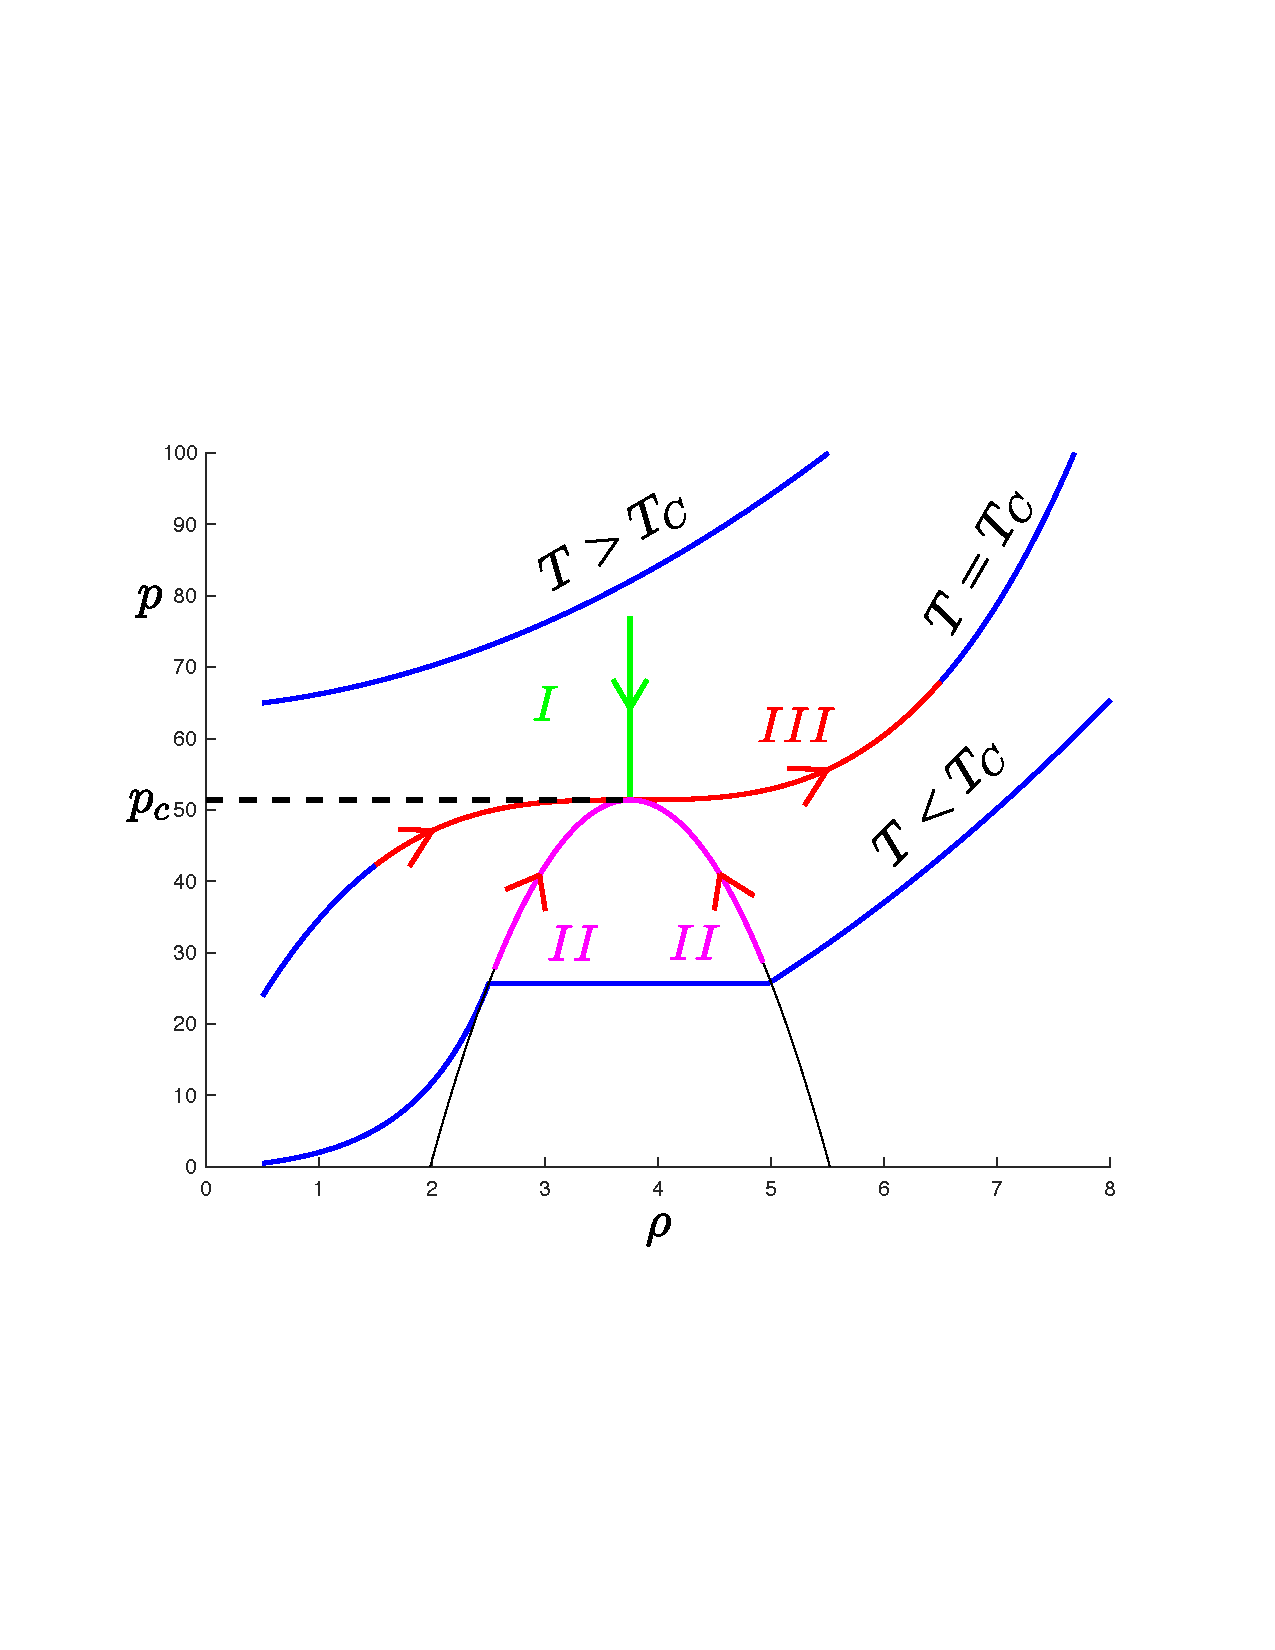
\includegraphics[width=10cm]{paths4pt}
\caption{{\bf Pressure versus density. Paths for the definition of the critical exponents.}}
%\label{}
\end{center}
\end{figure}



\begin{enumerate}
	\item Heat capacity ($\alpha:_{\pm}$) for real gases 
%
\begin{align}\label{eq:heat:capacity}
C_{V}&\simeq A_{\pm} \abs{\varepsilon}^{-\alpha_{\pm}}
:\qquad\begin{cases}
- &\text{for path II, i.e. } T \nearrow 	T_{c}, \text{with } \rho=\rho_{g,fl}\\
+ &\text{for path I, i.e. } T \searrow 	T_{c}, \text{with } \rho=\rho_{c}
\end{cases}\;.
\end{align}
%
Heat capacity ($\alpha',\alpha$) for magnets
\begin{align}\label{eq:}
C_{B}&\simeq  A_{\pm} \abs{\varepsilon}^{-\alpha_{\pm}}
:\qquad \begin{cases}
- & T \nearrow 	T_{c}, \text{with } B=0\\
 + &\text{for path I, i.e. } T \searrow 	T_{c}, \text{with } B=0
\end{cases}\;.
\end{align}
The experiment yields $\alpha_{\pm}\approx 0$. Ising 2D, exact solution, logarithmic divergence, i.e. $\alpha_{\pm}=0$. 
{\color{blue}(see section \ref{sec:Ising:2D:spec:heat}).}
Classic theories (i.e. Weißferrro-magnet, vdW gas) yield discontinuity,
which is equivalent to $\alpha_{\pm}=0$.
\item Order parameter ($\beta$ [not inverse temperature!]). A variable that exists only below $T_{c}$ and which characterises the order of the system.
E.g. magnetization $M$ or the for real gases the density difference 
$\Delta \rho = \rho_{fl}-\rho_{g}$, or rather $\Delta \rho = \rho_{fl,g}-\rho_{c}$, in the 
two-phase region
%
%
\begin{align}\label{eq:}
\frac{\Delta \rho(T)}{2 \rho_{c}} \simeq B|\varepsilon|^{\beta}&\;,\text{along path II}\\
\frac{M(T)}{M(0)} \simeq B|\varepsilon|^{\beta}&\;,\text{for zero magnetic field} \;.
\end{align}
%
The normalizations are introduced to make sure that $B$ is $O(1)$.
In principle, $\beta$ should be $\beta'$, as we are below $T_{c}$, but since the order parameter 
is only defined below $T_{c}$, it is common to use $\beta$. Typical experimental values are $0.35\pm 0.02$. classical theories yield $\beta=1/2$. 2D Ising exact, $\beta=1/8$. {\color{blue}(See section \ref{sec:Ising:2D:beta}).}
For the 3D Ising model one finds $\beta=0.325\pm 0.001$. While 3D Heisenberg gives $\beta=0.3445\pm 0.002$.

\item Compressibilities and susceptibilities ($\gamma_{\pm}$)


%
\begin{align*}
\kappa_{T} &= -\frac{1}{V}\pder{V}{p}{T} = \frac{1}{\rho} \pder{\rho}{p}{T}\;,\\
\chi_{T} &= \pder{M}{B}{T}
\end{align*}
%
\begin{align}\label{eq:}
\frac{\kappa_{T}}{\kappa^{0}_{T_{c}}}&\simeq C_{\pm} \abs{\varepsilon}^{\gamma_{\pm}}
:\qquad \begin{cases}
- &\text{for path II, i.e. } T \nearrow 	T_{c}, \text{with } \rho=\rho_{g,fl}\\
 + &\text{for path I, i.e. } T \searrow 	T_{c}, \text{with } \rho=\rho_{c}
\end{cases}\;.
\end{align}
%
Here $\kappa^{0}_{c}$ is the compressibility of the ideal gas at $T=T_{c}$, which follows (due to $\rho=\frac{p}{k_{B}T}$) from
%
\begin{align*}
\kappa &= \frac{1}{\rho} \frac{1}{k_{B}T} = \frac{1}{p}\;.
\end{align*}
%
Similarly, one uses for the normalization in the magnetic case, the result of an ideal paramagnet
%
\begin{align*}
M &=\frac{C^{*}}{T}\;,
\end{align*}
%
with $C^{*}$ being the Curie constant.
\begin{align}\label{eq:}
\frac{\chi_{T}}{\chi^{0}_{T_{c}}}&\simeq C_{\pm} \abs{\varepsilon}^{-\gamma_{\pm}}
:\qquad \begin{cases}
-&\text{for path II, i.e. } T \nearrow 	T_{c}, \text{with } H=0\\
 +&\text{for path I, i.e. } T \searrow 	T_{c}, \text{with } H=0
\end{cases}\;.
\end{align}
%
Typical experimental values differ somewhat about $\gamma\approx \gamma' \approx 1.3$.
Model calculations all yield $\gamma=\gamma'$. Classical models $\gamma=1$, 2D Ising exact,
$\gamma =7/4$, 3D Ising $\gamma\approx 1.24$, 3d Heisenberg $\gamma=1.39$.

\item Critical isotherm ($\delta$)
We define the critical pressure of the ideal gase as the pressure of the ideal gas at $T_{c}$ and 
$\rho_{c}$ via the ideal gas law
%
\begin{align*}
p_{c}^{(0)}&= k_{B}T_{c} \rho_{c}
\end{align*}
%
which clearly differs from the relation of the vdW model (see \eq{eq:p:cr}).
For the real gas we define the isothermal critical exponent as
%
\begin{align}
\frac{p-p_{c}}{p_{c}^{0}} & \simeq D \bigg| \frac{\rho-\rho_{c}}{\rho_{c}}\bigg|^{\delta} \text{sign} (\rho-\rho_{c})\;;\quad \big(\text{along the path III, } T=T_{c}  \big)\;.
\end{align}
%
If we define 
%
\begin{align*}
B_{C}^{(0)} &= \frac{k_{B} T_{c}}{\mu_{0} m}\;m
\end{align*}
%
with $m$ being the magnetic moment  per particle, then the corresponding relation for magnets reads
%
\begin{align*}
\frac{B}{B_{C}^{(0)}} &\simeq D \bigg|
\frac{M(T=T_{c},B)}{M(T=0,B=0)}
\bigg|^{\delta} \;\text{sign} (M)\;.
\end{align*}
%
Experimental values are in the range $\delta\in (4,5)$. The 2D Ising model yields $\delta=15$, which 
far off. The 3D Ising and Heisenberg model yields $\delta=4.9$ (much better). Classical theories 
yield $\delta=3$.

\item Correlation lengths ($\nu,\nu',\eta$)


We define a pair-correlation function, e.g. density-density or spn-spin,
%
\begin{align}
g(\vv r,\vv r') &= \avg{\Delta \rho(\vv r) \Delta \rho(\vv r')}\\
g_{ij} &= \avg{\Delta \vv S_{i} \Delta \vv S_{j}}\;.
\end{align}
%
In the critical regions they behave approximately like
%
\tboxit{Ornstein-Zernike function}{
\begin{align}\label{eq:Ornstein:Zernike}
g(\vv r,\vv r') &=c_{0}\;\frac{e^{-\frac{|\vv r - \vv r'|}{\xi(T)}}}{\abs{\vv r-\vv r'}}\\
g_{ij} &= g(\vv r_{i},\vv r_{j}) \;,
\end{align}}
%
with $\xi(T)$ is the correlation length.
It diverges on approaching the critical point.
For real gases one defines
%
\begin{align}\label{eq:}
\xi\simeq D_{\pm} \abs{\varepsilon}^{-\nu_{\pm}}
:\qquad \begin{cases}
-&\text{on path II}\;,\\
+&\text{on path I}\;.
\end{cases}
\end{align}
%
For magnets
\begin{align}\label{eq:}
\xi\simeq D_{\pm} \abs{\varepsilon}^{-\nu_{\pm}}
:\qquad
\begin{cases}
-	&\text{for }	T\nearrow T>T_{C}, B=0	\;,\\
+			&\text{for }	T\searrow T>T_{C}, B=0	\;.
\end{cases}
\end{align}
%
%
Finally, we also introduce the  pair-correlation function at the critical temperature $T=T_{c}$. According to the Ornstein-Zernike formula
in \eq{eq:Ornstein:Zernike}, at $T=T_{c}$ the correlation length is infinite and, therefore, the pair-correlation would decrease like
$1/\abs{\vv r-\vv r'}$. This is, however, not the case for real systems.
The behaviour is slightly different and expressed by
%
\begin{align*}
g(\vv r,\vv r') &=\big|\vv r-\vv r'\big|^{-(d-2+\eta)}
\begin{cases}
p=p_{C}  &\text{, real gases}\;,\\
B=0\text{, magnets}\;.
\end{cases}
\end{align*}
%
The Ornstein-Zernike formula would imply $\eta = 3-d$. For the other critical exponents $\nu,\nu'$ the deviation  from the $1/r$ dependence is negligible, as the the correlation length is obtained
from the slope of a fit of 
%
\begin{align*}
\ln(g(r)) &= c_{0} -\frac{r}{\xi(T)} - (d-2+\eta)\ln(r)
\end{align*}
%
versus $r$. Here the last term enters only logarithmically in $r$.




\end{enumerate}


\subsection{Scaling laws}
\blue{Generalized homogeneous functions} $f(x,y,\ldots)$ in several variables have the 
following property for arbitrary real $\lambda$
%
\begin{align}\label{eq:}
f(\lambda^{a_{x}} x,\lambda^{a_{y}}y,\ldots ) &=\lambda f(x,y,\ldots)\;,
\end{align}
%
where $a_{x},a_{y},\ldots$ can be any real numbers. An example would be
%
\begin{align*}
f(x,y) &= 4 x^{3} + 7 y^{8}\;,
\end{align*}
%
with $a_{x}=1/3$ and $a_{y}=1/8$, while 
%
\begin{align*}
f(x,y) &= x + 6 x^{2} + xy + y^{5}
\end{align*}
%
is no generalized homogeneous function. Next we will define the
{\color{blue}scaling hypothesis} in the case of the free energy $F(T,B)$ of a magnetic system. We are only interested in the non-analytic parts of $F$
near $T_{C}$ which we denote by
$F(\varepsilon,B) $.

\tboxit{Scaling hypothesis}{
%
\begin{align}\label{eq:}
F(\lambda^{a_{\varepsilon}}\varepsilon,\lambda^{a_{B}}B) &=
\lambda \;F(\varepsilon,B)\;.
\end{align}
%
}
This is not yet strictly proven in general, but there are many important
cases where the scaling hypothesis is fulfilled.

Now we can use the scaling hypothesis to express the critical exponents
in terms of the scaling parameters $a_{\varepsilon}$ and $a_{B}$.
Differentiation w.r.t. $B$ yields
%
\begin{align*}
 \frac{\partial }{\partial b}
 F(\lambda^{a_{\varepsilon}}\varepsilon,b) \bigg|_{b= \lambda^{a_{B}}B}
\; \lambda^{a_{B}}
&\overset{!}{=} \lambda
\frac{\partial }{\partial B}
F(\varepsilon,B)\;.
\end{align*}
%
Now we have 
%
\begin{align*}
M &= -\frac{\partial F}{\partial B}
\end{align*}
%
and therefore  we have
%
\begin{align}
\lambda^{a_{B}} 
M(\lambda^{a_{\varepsilon}}\varepsilon,\lambda^{a_{B}}B) 
&= \lambda M(\varepsilon,B)\;.
\end{align}
%
\begin{enumerate}
	\item[a)] {\color{blue}Exponent $\beta$:} We use $B=0$ and obtain
%
\begin{align*}
\lambda M(\varepsilon,0) &=M(\lambda^{a_{\varepsilon}}\varepsilon,0) \;,
\end{align*}
%
which is valid for any $\lambda$, also for 
%
\begin{align*}
\lambda&=(-\varepsilon)^{-1/a_{\varepsilon}}\;,
\end{align*}
%
resulting in 
%
\begin{align*}
M(\varepsilon,0) &= (-\varepsilon)^{\frac{1-a_{B}}{a_{\varepsilon}}} M(-1,0)\simeq (\varepsilon)^{\frac{1-a_{B}}{a_{\varepsilon}}} \;.
\end{align*}
%
Hence, 
%
\begin{align*}
\beta=\frac{1-a_{B}}{a_{\varepsilon}} \;.
\end{align*}
%
\item[b)] {\color{blue}Exponent $\delta$ (critical isotherm):}
Next we use $\varepsilon=0$ and have
%
\begin{align*}
M(0,B) &= \lambda^{a_{B}-1}\;M(0,\lambda^{a_{B}}B)\;.
\end{align*}
%
Here we choose $\lambda =B^{-1/a_{B}}$ and obtain
%
\begin{align*}
M(0,B) &\simeq  B^{\frac{1-a_{B}}{a_{B}}}\\
B &\simeq M^{\frac{a_{B}}{1-a_{B}}}\;,
\end{align*}
%
and hence $\delta=\frac{a_{B}}{1-a_{B}}$.
In summar, we have
%
\begin{align}\label{eq:}
a_{B} &= \frac{\delta}{1+\delta}\\
a_{\varepsilon} &= \frac{1}{\beta}\frac{1}{1+\delta}\\
\end{align}
%
\end{enumerate}
We can express further critical exponents in terms of the scaling parameters, which then in turn allows to find relations among the 
critical exponents:
%
From the scaling laws one finds
\begin{align}
\alpha&=\alpha'\;;\quad
\gamma=\gamma'\;;\quad\nu=\nu'\;.
\end{align}
%
and also
%
\begin{align}
\alpha+2\beta+\gamma &=2\\
\alpha+\beta (1+\delta)&=2\\
\beta &=\frac{\gamma}{\delta-1}\\
\nu &=\frac{\gamma}{2-\eta}\;.
\end{align}
%

